\pdfminorversion=7 % avoid warning: "PDF inclusion: found PDF version <1.7>, but at most version <1.5> allowed"
\documentclass[a4paper]{article}


%% ----- Packages -----

% Language and Character encoding
\usepackage[english]{babel}
\usepackage[utf8]{inputenc}
\usepackage[T1]{fontenc}

% Math Symbols
\usepackage[fleqn]{amsmath} % fleqn to set the equations left
\usepackage{amssymb}
\usepackage{amsthm} 

% Standard Packages
\usepackage{paralist} % for compactitem und compactenum
\usepackage{ellipsis}
% \usepackage{fixltx2e} % fixltx2e is not required with releases after 2005(fixltx2e)
\usepackage{lmodern} % Latin Modern
\frenchspacing

\usepackage[final]{microtype}
\usepackage{amsfonts}
\usepackage{booktabs}
\usepackage{graphicx}
\usepackage{epstopdf} % necessary using MikTeX
\usepackage{epigraph}
\usepackage{xspace}
\usepackage{bm}
\usepackage{marginnote}
\usepackage{subcaption}
\usepackage{caption}
\captionsetup[subfigure]{labelformat=simple}
\captionsetup{font=small,labelfont={bf,sf}}
\captionsetup[sub]{font=small,labelfont={sf}}
\renewcommand\thesubfigure{(\alph{subfigure})}

% Additional Optional Packages
%\usepackage[notcite,notref]{showkeys} % Show names of labels
\usepackage{changes} % \added{...}, deleted{...} or \replaced{great}{small}
\usepackage{nth}     % oridinal numbers: 1st, 2nd, ... by \nth{1}, \nth{2}, ...
                     % \usepackage[super]{nth} % Option 'super' not available at University
\usepackage{enumitem}
\usepackage{dsfont}
\usepackage{xcolor}
\usepackage{accents}
\usepackage{url} \urlstyle{sf} 
\usepackage[per=frac,fraction=frac]{siunitx} %\si{...} units...
\usepackage{wrapfig}
\usepackage{capt-of}
\usepackage{xspace} % dynamic space
\usepackage{multicol}
\usepackage{minibox}
%\usepackage{enumerate}
%\usepackage{bookmark}

\usepackage{tikz}

\usepackage{longtable} % \begin{longtable} ... breaks the table in case of pagebreak (instead of tabular)

\usepackage{ltablex}   % tabularx instead of tabular environment possible with pagebreak...
% Instead of: \begin{tabular}[t]{p{2.4cm} p{13.2cm}} (No pagebreak)
% Use:  \begin{tabularx}{\linewidth}{p{2.4cm} p{13.2cm}} (automatic pagebreak)

\usepackage{textcomp} % required for option upquote=true in lstset

% inline equation number
\newcommand*{\ineqno}[1]{\refstepcounter{equation}\label{#1}(\theequation)}

\usepackage{listings}
% MATLAB environment for source code in lstlisting
\lstloadlanguages{Matlab}
\lstset{%
float=ht, % float does not work globally..., see workaround below
basicstyle={\small\sffamily}, % alternative: ttfamily
literate=*{*}{\normalfont{*}}1, % Solution of the problem that asterik is vertically centered
columns=fullflexible, % fullflexible, flexible and fixed
frame=tb,
% language=Matlab,
upquote=true, % Simple quotes in source code are the correct ones... (otherwise MATLAB error...)
numbers=left,
numberstyle={\tiny},
showstringspaces=false,
captionpos=b, % lstlisting: define position of caption
keepspaces=true
}
% float workaround:
\makeatletter
\let\lst@floatdefault\lst@float
\makeatother

\usepackage{hyperref} % last package: exceptions: geometry, dblaccnt
\hypersetup{
pdftitle = {User Guide for IPscatt},
pdfsubject = {},
pdfauthor = {Florian B\"urgel, Kamil S. Kazimierski, and Armin Lechleiter},
pdfkeywords = {Inverse Scattering Problem, Sparsity Regularization, Total Variation, Primal-Dual Algorithm, MATLAB Toolbox IPscatt},
colorlinks = true, allcolors = blue, % true/false
%hidelinks, % all links hidden...
draft = false} % true/false

% \usepackage[width=16.5cm,top=2.25cm]{geometry} % load it after hyperref
\usepackage[width=16.5cm,top=3cm,bottom=4cm]{geometry} % load it after hyperref
\usepackage{dblaccnt} % load it after hyperref (before produces errors...)

%% ----- Declare Colors -----

\definecolor{blue}{rgb}{0,0,0.8}
\definecolor{green}{rgb}{0,0.5,0}
\definecolor{red}{rgb}{1,0,0}
\definecolor{orange}{rgb}{1,0.55,0}
\definecolor{gray}{rgb}{0.3,0.3,0.3}
% Commands for colors: note that {{...}} is important, otherwise the rest of the document is colored...
\newcommand{\blue}[1]{{\color{blue}{#1}}}   % \blue{...}
\newcommand{\green}[1]{{\color{green}{#1}}} % \green{...}
\newcommand{\red}[1]{{\color{red}{#1}}}     % \red{...}
\newcommand{\orange}[1]{{\color{orange}{#1}}}     % \orange{...}
\newcommand{\gray}[1]{{\color{gray}{#1}}}     % \grey{...}

% ----- Colors in Table -----
\usepackage{colortbl} % e. g. \cellcolor{gray}{0.9}
\newcommand{\highcol}{\cellcolor{gray!10}}

%% ----- Document specific -----

%\setlength{\parindent}{0in} % no indentation % suppress it with \noindent at the beginning of a line, e.g. \noindent\begin{tabular} is very useful
% \setlength{\mathindent}{0pt} % no indent for formulas, default: 15pt
\setlength{\marginparwidth}{2 cm}
% \pagestyle{headings}

% Renew itemize (smaller space between lines)
\let\tempone\itemize
\let\temptwo\enditemize
\renewenvironment{itemize}{\tempone\addtolength{\itemsep}{-0.5\baselineskip}}{\temptwo}

% Footnotes
\renewcommand*{\thefootnote}{\fnsymbol{footnote}} % Symbols for footnotes (instead of numbers)
%\renewcommand*{\thefootnote}{\arabic{footnote}} % default: switch back to arabic numbering in footnotes

%% ----- Declare Theorems -----

\theoremstyle{definition}
\newtheorem{defi}{Definition}[section] % definition
\newtheorem{prob}[defi]{Problem}       % problem
\newtheorem{exam}[defi]{Example}       % example
\newtheorem{algo}[defi]{Algorithm}     % algorithm
\theoremstyle{plain}
\newtheorem{rema}[defi]{Remark}        % remark
\newtheorem{theo}[defi]{Theorem}       % theorem
\newtheorem{lemm}[defi]{Lemma}         % lemma
\newtheorem{coro}[defi]{Corollary}     % corollary

%% ----- Symbols -----
\newcommand*{\formc}{\framebox[0.4cm]{\textsf{C}}}  % continuous formula
\newcommand*{\formd}{\framebox[0.4cm]{\textsf{D}}}  % discretized formula
\newcommand*{\forms}{\framebox[0.4cm]{\textsf{S}}}  % source code

%% ----- Definitions and commands... -----

% Declare Mathematical Operators
\DeclareMathOperator*{\argmin}{arg\,min}
\newcommand*{\real}{\mathrm{Re}}  % real part (\Re is defined yet)
\newcommand*{\imag}{\mathrm{Im}}  % imaginary part (\Im is defined yet)

% Declare Mathematical Sets
\newcommand*{\R}{\mathbb{R}}      % real numbers
\newcommand*{\C}{\mathbb{C}}      % complex numbers
\newcommand*{\N}{\mathbb{N}}      % natural numbers
\newcommand*{\Z}{\mathbb{Z}}      % set of all integers
\newcommand*{\K}{\mathbb{K}}
\renewcommand{\S}{\mathbb{S}}     % unit sphere

% Declare Mathematical Symbols
\newcommand{\im}{\mathrm{i}}    % imaginary unit i
\newcommand{\e}{\mathrm{e}}     % exponential function
\newcommand{\adj}{\mathrm{H}}	% adjoint matrix is hermitian matrix: use A^\adj
% Note: transpose: A^\top

% Declare Mathematis: Integral
\newcommand{\dif}{\mathrm{d}}
\renewcommand*{\d }[1]{\thinspace \dif #1} % call: $\int_0^x g(y) \d{y}$

% IPscatt: mathcal
\newcommand{\F}{\mathcal{F}}  % forward operator
\newcommand{\G}{\mathcal{G}}  % grid
\newcommand{\HM}{\mathcal{H}} % harmonic monomial (hmonomial in matchIncField.m)
\newcommand{\V}{\mathcal{V}}  % matrix V: \V c \approx u^\Inc|_{\Gamma_\Sca}.
% \newcommand{\Mul}{\mathcal{M}} % multi-static (not used)

% IPscatt: Operators
\newcommand{\grad}{\operatorname{grad}} % gradient
\newcommand{\dive}{\operatorname{div}}  % divergence
\newcommand{\supp}{\operatorname{supp}} % support

\newcommand{\SL}{\operatorname{SL}}        % single-layer
\newcommand{\LipS}[1]{T_{#1}}              % Symbol for the Lippmann-Schwinger Operator
\newcommand{\LipSd}[1]{T_{#1}}             % Symbol for the discretized LS-Operator

\newcommand{\iproj}[1]{\mathcal{I}_{[#1]}} % Interval projection
\newcommand{\stepf}[1]{\text{step}_{[#1]}} % Step function

% IPscatt
\newcommand{\ROI}{{D}}                % region of interest (ROI): (continuous) D
\newcommand{\CD}{{D_{2R}}}            % computational domain (CD): (continuous) D_{2R}
\newcommand{\ROID}{\C^{N_\mathrm{D}}} % region of interest (ROI): discretized: C^{N_D} (N_D is \NROI)
\newcommand{\CDD}{\C_N^d}             % computational domain (CD): discretized: C_N^d
\newcommand{\ROIS}{\textsf{ROI}}      % region of interest (ROI): pseudocode: \textsf{} sf... s... (code: seti.gridROI)
\newcommand{\CDS}{\textsf{CD}}        % computational domain (CD): pseudocode: \textsf{} sf... s... (code: seti.grid)

\newcommand{\TX}{{\Gamma_\Inc}}       % transmitters: (continuous) \Gamma_i
\newcommand{\RX}{{\Gamma_\Sca}}       % receivers: (continuous) \Gamma_s
\newcommand{\TXD}{\C^{N_\Inc}}        % transmitters: discretized: C^{N_i}
\newcommand{\RXD}{\C^{N_\Sca}}        % receivers: discretized: C^{N_s}
\newcommand{\TXS}{\textsf{incPnts}}   % transmitters: pseudocode: incPnts
\newcommand{\RXS}{\textsf{measPnts}}  % receivers: pseudocode: measPnts
\newcommand{\TXM}{\mathrm{TX}}   % transmitters: mathrm TX
\newcommand{\RXM}{\mathrm{RX}}   % receivers: mathrm RX

\newcommand{\dS}{\mathrm{dS}}  % approximation of the infinitesimal element
\newcommand{\dV}{h_N^d}        % area/volume of the infinitesimal element (pixel/voxel) of CD

% IPscatt: norms and inner products
\newcommand{\HS}{\mathrm{HS}}       % Hilbert-Schmidt norm
\newcommand{\fro}{\mathrm{F}}       % Frobenius norm
\newcommand{\WS}{\mathrm{dis}}      % norm of discrepancy term..., and corresponding inner product
\newcommand{\sparse}{\mathrm{spa}}  % norm of sparsity penalty
%\newcommand{\spa}{\mathrm{roi}}    % norm of sparsity penalty, was deleted
\newcommand{\TV}{\mathrm{tv}}       % norm of total variation (TV) penalty (fg)
\newcommand{\normROI}{\mathrm{roi}} % norm of ROI

% IPscatt: names of penalty terms
\newcommand{\dis}{\mathrm{dis}}    % discrepancy: f_dis
\newcommand{\gra}{\mathrm{tv}}     % total variation penalty (in code: gra)
\newcommand{\phy}{\mathrm{phy}}    % penalty for physical bounds

% IPscatt: auxiliary to penalty terms
\newcommand{\SpaPhy}{\mathrm{rp}}  % v_rp alt: _{sp}

% IPscatt: fields
\newcommand{\Inc}{\mathrm{i}} % incident field u^i as well as transmitters' positions
\newcommand{\Sca}{\mathrm{s}} % scattered field u^s as well as receivers' positions, e. g. u^\Inc|_{\Gamma_\Sca}
\newcommand{\Tot}{\mathrm{t}} % total field u^t

% IPscatt: forward scattering
\newcommand{\msdata}{F_\mathrm{meas}} % multi-static data (the data) (at receivers' positions)
% \newcommand{\NROI}{N_{\mathrm{D}}}  % f_\NROI results in an error: ``Double subscript''; It works with f_{\NROI} or additional brackets in defintion of newcommand
\newcommand{\NROI}{{N_{\mathrm{D}}}}  % number of grid points in ROI
\newcommand{\shi}{\mathrm{shi}}       % shift

% IPscatt: names
\newcommand{\FFT}{\mathrm{FFT}} % FFT: Fast Fourier transform

% IPscatt: subindexes for iteration
\newcommand{\inn}{\mathrm{in}}  % inner iteration
\newcommand{\out}{\mathrm{out}} % outer iteration

% IPscatt: Convex Analysis
\newcommand{\fenchel}{\ast} % Fenchel conjugate symbol

% IPcatt: Identify complex and real matrices 
\newcommand{\CtoR}{\mathrm{T}}      % complex to real
\newcommand{\RtoC}{\mathrm{T}^{-1}} % real to complex

% IPscatt: Fourier transform
\newcommand{\factorKernel}{\Psi_{2R}}              % Fourier coefficients in the definition of V_2R
\newcommand{\factorKernelN}{\Psi_{N}}              % array of Fourier coefficients in V_N_D
\newcommand{\factorKernelNshi}{\widehat{\Phi}_{N}} % shifted version of Fourier coefficients

% IPscatt: Operator Symbols
\newcommand{\pmul}{\odot{}}        % element-wise multiplication
\newcommand{\pmulop}[1]{(#1\pmul)} % operator of element-wise multiplication

% IPscatt: Other mathrm...
\newcommand{\x}{\mathrm{x}}
\newcommand{\y}{\mathrm{y}}
\newcommand{\mat}{\mathrm{Mat}}
\newcommand{\born}{\mathrm{B}}

% IPscatt: Names in Text
\newcommand{\IPscatt}{\textsf{IPscatt}\xspace} % toolbox's name: \textsf{tboxIPscatt} and dynamic space
\newcommand{\MATLAB}{\textsf{MATLAB}\xspace}



\begin{document}

\title{\Large User Guide for \IPscatt---a \MATLAB Toolbox for the Inverse Medium Problem in Scattering}

\author{
Florian B\"urgel\footnote{University of Bremen, Center for Industrial Mathematics, Germany,
\textsf{\href{mailto:fbuergel@uni-bremen.de}{fbuergel@uni-bremen.de}}.}, \quad
Kamil S. Kazimierski\footnote{University of Graz, Institute of Mathematics and Scientific Computing, Austria, \textsf{\href{mailto:kazimier@uni-graz.at}{kazimier@uni-graz.at}}. The Institute of Mathematics and Scientific Computing is a member of NAWI Graz (\url{www.nawigraz.at}) and BioTechMed Graz (\url{www.biotechmed.at}).}, \quad
Armin Lechleiter\footnote{University of Bremen, Center for Industrial Mathematics, Germany.}
}

\date{User Guide for Release \textsf{ipscatt2017}, updated \today}

\maketitle

\begin{abstract}
\IPscatt is a free, open-source \MATLAB toolbox facilitating the solution of the two and three-dimensional inverse medium problem in time-independent scattering (also known as time-harmonic scattering).
%
For a survey of the mathematical concepts beyond the provided implementation we refer to the corresponding \emph{algorithm paper}. In particular, the \emph{algorithm paper} describes the direct scattering problem and the implemented variational reconstruction scheme.
%
This \emph{user guide} contains installation instructions, a technical description, practical guides for using the library with code snippets as well as resulting figures and finally some applications.
\end{abstract}

{\small \paragraph{Keywords} Inverse Scattering Problem, Parameter Identification, \MATLAB Toolbox, Denoising, Sparsity Regularization, Total Variation Regularization, Primal-Dual Algorithm, User Guide.}

\tableofcontents

%%

\section*{Introduction}

Inverse medium problems in scattering attempt to identify the contrast, that is the squared refractive index minus one, of a penetrable medium from measurements of waves scattered from that medium. This parameter identification problem has many interesting application areas, e.g. in non-destructive testing procedures. As a nonlinear and ill-posed problem it is challenging, although we limit ourselves to time-independent scattering; the huge system sizes after discretization makes the problem even more demanding.
%
Therefore we provide the free, open-source software \IPscatt, which is an efficient and effective \MATLAB toolbox for the nonlinear inverse medium problem in time-independent scattering in two and three dimensions.
%
The variational regularization scheme, on which the reconstruction part of \IPscatt is based, minimizes the defect and the penalty terms that take into account a~priori information. This scheme was introduced in \cite[Sec.~4]{Buergel2017} and relies on the so-called primal-dual algorithm due to Pock, Bischof, Cremers and Chambolle, see~\cite{Pock2009, Chambolle2011}. To the authors' best knowledge, \IPscatt is the first toolbox that combines sparsity promoting and total variation-based regularization to jointly improve the reconstruction quality. Further, physical bounds are used as a~priori information on the scattering object restricting the real and imaginary part of the contrast.

This \emph{user guide} was written for readers, who are interested in using the software \IPscatt, and is part of the supplementary material\footnote{Supplementary material is provided on \url{https://calgo.acm.org/} and on \url{http://www.fbuergel.de/ipscatt/} in the latest version.}, which contains first, the \emph{source code}, second, this \emph{user guide} and third, the \emph{source code documentation} containing a detailed description of each function.

Also, an \emph{algorithm paper} for \IPscatt was written, which contains an overview of the software framework, presents its key features, describes the direct scattering problem as well as the underlying variational reconstruction scheme, compares \IPscatt with other software packages and discusses the application areas.

\paragraph{Organization of this User Guide} This \emph{user guide} is organized as follows: 
Sec.~\ref{sec:installation} contains some general information about the software, installation instructions and the first code snippet to demonstrate a typical work flow. 
Then, the technical description containing a typical program flow and the most important variables is given in Sec.~\ref{sec:tech}. 
Next, we show the main functionality of \IPscatt on selected examples in Sec.~\ref{sec:guidelines}. 
The modular design of \IPscatt is shown on selected examples in Sec.~\ref{sec:applications}. We hope this encourages users of \IPscatt to take parts of it and use them for their own applications. 
For the reader's convenience we repeat some formulas from the \emph{algorithm paper} in the Appendix if we refer to them, in particular from the direct scattering problem and the implemented reconstruction scheme. 
Further, in the Appendix we repeat the continuous and discretized forms of the direct scattering problem from the \emph{algorithm paper} in a tabular and also give them in the source code form to build a connection between mathematical formulas and their implementation.

%%

\section{Installation}\label{sec:installation}

This section contains the metadata of the software, installation instructions and a first demonstration of the toolbox. Furthermore, we give a first code snippet to present a typical work flow and refer to the most important guides for a quick introduction to the toolbox \IPscatt.

\paragraph{Software Metadata} The software package \IPscatt is a \MATLAB toolbox for the inverse medium problem in time-independent scattering. It is provided as free software under the GNU General Public License (GPLv3). 
The toolbox is written in \MATLAB and is therefore supported on any operating system which \MATLAB supports. It was extensively tested in \MATLAB R2016b under Linux, but short tests under Windows~7 and~10 were also successful. Apart from \MATLAB the software library \IPscatt depends on the ``Signal Processing Toolbox'' and the ``Image Processing Toolbox''. Unfortunately, \IPscatt does not work with Octave (at least in version 4.0.0). 
As already mentioned we provide as supporting material, apart from this \emph{user guide}, a \emph{source code documentation} containing a detailed description of each function.

All computations in this \emph{user guide} were carried out on a workstation with an Intel(R) Core(TM) i7-3770 CPU with 3.40\,GHz and 32\,GByte RAM. 
For the given code snippets we recommend more than 5\,GByte RAM. This, in particular, is true for the three-dimensional reconstruction example as it is the most RAM-consuming one.

\paragraph{Installation}
For installation just unpack the compressed archive. It contains the folder \textsf{code} with the \emph{source code}, the folder \textsf{doc} with the \emph{source code documentation} and the folder \textsf{guide} with this \emph{user guide}. The directory structure of \textsf{code} is described in the following list.

\setlength{\columnseprule}{0.25pt}
\setlength{\columnsep}{10pt}
\begin{multicols}{2}[][10mm]
\begin{compactitem}
  \item \textsf{3rdparty} (\nth{3} party code)
  \item \textsf{conv} (convenience functions)
  \item \textsf{docCreate} (creates the documentation)
  \item \textsf{guides} (code for the guides)
  \item \textsf{incontrasts} (input of predefined contrasts)
  \item \textsf{inseti} (input of structure array \textsf{seti})
  \item \textsf{output} (place to store files and figures)
  \item \textsf{proc} (process)
  \begin{compactitem}
   \item \textsf{auxi} (auxiliary routines)
   \item \textsf{expData} (working with real-world data)
   \item \textsf{expSetup} (experimental set-up)
   \item \textsf{intOps} (integral operators)
   \item \textsf{norms} (definitions of norms)
   \item \textsf{operators} (operators)
   \item \textsf{plots} (functions for plots)
   \item \textsf{plotsAux} (auxilary functions for plots)
   \item \textsf{recon} (reconstruction process)
   \item \textsf{reconAux} (associated auxiliary functions)
   \item \textsf{setData} (sets geometry and simulation)
   \item \textsf{setInput} (general input, e.g. make folders)
  \end{compactitem}
  \item \textsf{tests} (test functions)
  \begin{compactitem}
   \item \textsf{auxi} (auxiliary functions)
  \end{compactitem}
\end{compactitem}
\end{multicols}

\paragraph{Demonstration} For a first impression of \IPscatt we use the routine \textsf{demo} in \MATLAB with \textsf{code} as current folder. This executes a demonstration script in which all important parts of \IPscatt are executed. However, to keep the run time low the number of transmitters/receivers, discretization points and reconstruction steps was set very low. This means that the resulting reconstruction is not representative for \IPscatt. The generated figures are saved in a folder with the current date as prefix inside the directory \textsf{output}.

\paragraph{Quick Start and Typical Work Flow} Input parameters can be set in the fields of the structure array\footnote{We follow \MATLAB's nomenclature denoting an \emph{associative array} as \emph{structure array} and \emph{return values} as \emph{output arguments}.} \textsf{seti}, that is a mutable data structure. \IPscatt takes care that all necessary fields are set in a consistent manner, e.g. if these fields are empty as in Lst.~\ref{lst:quickStart}, default parameters will be set. In the routine to set the data, \textsf{setData}, this concerns e.\,g. the underlying grid, the positions of the transmitters and receivers, the type of the incident field as well as the predefined contrast of the scattering object. Furthermore, \textsf{setData} solves the direct scattering problem and adds Gaussian noise to the simulated data. In the end, the variational reconstruction starts by \textsf{recon} after reconstruction-dependent parameters were set in \textsf{setRecon}.
\begin{lstlisting}[caption={Quick Start Example.},label=lst:quickStart]
init;
seti = struct; seti = setData(seti);
seti = setRecon(seti); seti = recon(seti);
\end{lstlisting}

For a quick introduction to the toolbox \IPscatt see the guides in Sec.~\ref{sec:guidelines}, in particular Sec.~\ref{sec:guide:setGrid}, \ref{sec:guide:expSetup}, \ref{sec:guide:contrast}, \ref{sec:guide:setGeomSim}, \ref{sec:guide:addNoise} and~\ref{sec:guide:recon}. These guides will show how to: generate a grid; use some standard transmitter-receiver geometries for the experimental set-up; 
load predefined contrasts; 
set geometry and simulation easily; 
simulate data with noise; 
reconstruct in the case of two and three-dimensional scattering.

%%

\section{Technical Description}\label{sec:tech}

The typical program flow of \IPscatt is visualized in Fig.~\ref{fig:flowChart}, in which the right column contains the code of a typical work flow. Optional parts of \IPscatt are shown in Fig.~\ref{fig:flowChartOptional}. Furthermore, the most important fields of the structure array \textsf{seti} are listed in Tab.~\ref{tab:impFields}. We will take a closer look at some of the functions and fields in the guides in Sec.~\ref{sec:guidelines}. However, a detailed reference of all existing functions is in the \emph{source code documentation}.
%
In particular, this \emph{source code documentation} is interesting for advanced usage and further development of \IPscatt for which the toolbox was designed. Therefore \IPscatt supports the user by providing tests of internal functions. In particular, it tests the proper working of the forward operator and its derivative. These tests may take a long time and are started by \textsf{seti = runtests()} with \textsf{code} as current folder.

\begin{figure}
\hrulefill

\textbf{Function: \textsf{setGeomSim.m}}, see Sec.~\ref{sec:guide:setGeomSim} (geometry and simulation):

\begin{compactitem}
\item Grid (CD and ROI) (Sec.~\ref{sec:guide:setGrid}) (\textsf{setGrid.m} $\mapsto$ \textsf{seti.grid}, \textsf{seti.gridROI}).
\item Experimental set-up (Sec.~\ref{sec:guide:expSetup}):
 \begin{compactitem}
 \item Transmitters' positions (\textsf{setIncPnts.m} $\mapsto$ \textsf{seti.incPnts}).
 \item Receivers' positions (\textsf{setMeasPnts.m} $\mapsto$ \textsf{seti.measPnts}).
 \item Incident field (\textsf{setIncField.m} $\mapsto$ \textsf{seti.incField}).
 \item Measurement kernel (\textsf{setMeasKer.m} $\mapsto$ \textsf{seti.measKer}).
 \end{compactitem}
 \item Contrast (Sec.~\ref{sec:guide:contrast}) ($\mapsto$ \textsf{seti.qROIexact}).
\end{compactitem}

\hrulefill

%% ----- minipage: start -----

\begin{minipage}[t]{\dimexpr.24\textwidth-\tabcolsep-.5pt}
% -- Column 1 --
\centerline{\emph{Auxiliary routines}}
\vspace*{-0.2cm}

\hrulefill

\ \\ \\
\vspace*{-0.2cm}

\hrulefill

\bigskip
\bigskip
\bigskip

\textsf{setGeomSim.m}\\
(see above)

\bigskip

\textsf{forward.m}:

\begin{enumerate}[topsep=0mm, itemsep=0mm, parsep=0mm, leftmargin=3mm, labelsep=0.5mm]
 \item \textsf{init.m}.
 \item \textsf{setGeomSim.m}.
 \item \textsf{forward.m}, Sec.~\ref{sec:guide:forward}: \\ $\mapsto \textsf{FFqMeas} = \F(q)$.\\
 (Underlying: \textsf{mimo.m}.)
\end{enumerate}

\vspace{2.0cm}
\vspace*{-0.2cm}

\hrulefill

\bigskip

\textsf{forward.m}, \textsf{derivative.m}:

\begin{enumerate}[topsep=0mm, itemsep=0mm, parsep=0mm, leftmargin=3mm, labelsep=0.5mm]
 \item \textsf{init.m}.
 \item \textsf{setGeomSim.m}.
 \item \textsf{forward.m}, Sec.~\ref{sec:guide:forward}: \\ $\mapsto \textsf{FFqMeas} = \F(q)$\\ 
 or\\
 \textsf{derivative.m}, Sec.~\ref{sec:guide:derivative}: \\ $\mapsto$ \textsf{JA}, \textsf{JB} to compute $\F'(q)[h] = \textsf{JA*}h\textsf{*JB}$.\\
 (Underlying: \textsf{mimo.m}).
\end{enumerate}

\end{minipage}
\hfill\begingroup\color{gray}\vrule width 1pt\endgroup\hfill
\begin{minipage}[t]{\dimexpr.56\textwidth-\tabcolsep-.5pt}
% -- Column 2 --

\centerline{\emph{Main program}}
\vspace*{-0.2cm}

\hrulefill

\centerline{\textbf{\textsf{init.m}}}

\centering (Initialization, see Sec.~\ref{sec:guidelines})

\centering $\downarrow$
\vspace*{-0.2cm}

\hrulefill

\centering \textbf{\textsf{setData.m}}

\centering (Sec.~\ref{sec:guide:addNoise} and~\ref{sec:guide:matchIncField})

\medskip
\centering $\swarrow$ \hspace*{3cm} $\searrow$
\medskip

\begin{minipage}[t]{\dimexpr.5\textwidth-\tabcolsep-.5pt}
\centering \emph{Simulated data with noise} \\ \ 
\smallskip

\begin{enumerate}[topsep=0mm, itemsep=0mm, parsep=0mm, leftmargin=3mm, labelsep=0.5mm]
 \item \textsf{setGeomSim.m}, Sec.~\ref{sec:guide:setGeomSim}: \\ $\mapsto$~\textsf{seti.incField},\\ $\mapsto$~\textsf{seti.qROIexact}.
 \item \textsf{forward.m}, Sec.~\ref{sec:guide:forward}: \\ $\mapsto$~\textsf{seti.FmeasExact}.
 \item \textsf{addNoise.m}, Sec.~\ref{sec:guide:addNoise}: \\ $\mapsto$ \textsf{seti.FmeasDelta}.
\end{enumerate}
\end{minipage}
%
\hfill\begingroup\color{gray}\vrule width 0.5pt\endgroup\hfill
%
\begin{minipage}[t]{\dimexpr.5\textwidth-\tabcolsep-.5pt}
\centering \emph{Real-world data (Fresnel)}\\ (\textsf{loadData.m}, Sec.~\ref{sec:guide:matchIncField})
\smallskip

\begin{enumerate}[topsep=0mm, itemsep=0mm, parsep=0mm, leftmargin=3mm, labelsep=0.5mm]
 \item \textsf{readRAWData.m}, Sec.~\ref{sec:guide:workingFresnel}: \\ 
 (via \textsf{uTotRX}, \textsf{uIncRX}) \\ $\mapsto$~\textsf{seti.FmeasDelta}.
 \item \textsf{setGeomSim.m}.
 \item \textsf{matchIncField.m}, Sec.~\ref{sec:guide:matchIncField}:\\ 
 (via \textsf{uIncROI}) \\ $\mapsto$ \textsf{seti.incField}.
\end{enumerate}
\end{minipage}

\bigskip

\centering $\mapsto$ \textsf{seti.FmeasDelta}

\centering (data---simulated data with noise or real-world data)

\centering $\downarrow$
\vspace*{-0.2cm}

\hrulefill

\begin{center}
 
\textbf{\textsf{setRecon.m}}\\

(Sets required fields in \textsf{seti}, Sec.~\ref{sec:guide:recon}.)

$\mapsto$~\textsf{seti.alpha}, \textsf{seti.beta}, \textsf{seti.physBounds}.

\centering $\downarrow$

\textbf{\textsf{recon.m}}

(Variational reconstruction, Sec.~\ref{sec:guide:recon}.)

\addtolength{\fboxsep}{-1pt} % instead of setlength because can be corrected later
\fbox{
\addtolength{\tabcolsep}{-5pt}
\begin{tabular}[t]{p{2.6cm} p{2.1cm} p{1.9cm}}
\fbox{Inner iteration} & by \textsf{pda.m} & $\mapsto \textsf{h}$\\
\quad \quad \quad $\downarrow$ $\uparrow$ & &\\
\fbox{Outer iteration} & by \textsf{minPda.m} & $\mapsto q := q + h$\\
 & \multicolumn{2}{l}{(with $q = \textsf{seti.qROIcomp}$ and $h = \textsf{h}$).}
\end{tabular}
\addtolength{\tabcolsep}{+5pt}
}
\addtolength{\fboxsep}{+1pt} % instead of setlength because can be corrected later

\medskip

$\mapsto$ \textsf{seti.qROIcomp}\\
(Reconstructed contrast as a vector.)
\end{center}

\end{minipage}
\hfill\begingroup\color{gray}\vrule width 1pt\endgroup\hfill
\begin{minipage}[t]{\dimexpr.20\textwidth-\tabcolsep-.5pt}
% -- Column 3 --

\centerline{\emph{Code}}
\vspace*{-0.2cm}

\hrulefill

\ \\
\textsf{init;}
\ \\
\vspace*{-0.2cm}

\hrulefill

\ \\
\textsf{seti = struct;}

\textsf{seti = setData(seti);}

\vspace{5.75cm}

\hrulefill

\ \\
\textsf{seti = setRecon(seti);}

\textsf{seti = recon(seti);}

\end{minipage}

\hrulefill

%% ----- minipage: end -----


\caption{The typical program flow of \IPscatt with the most important output arguments (emphasized by~$\mapsto$).}
\label{fig:flowChart}
\end{figure}

\begin{figure}
\hrulefill\\
\textbf{Optional Parts of \IPscatt}
\begin{compactitem}
  \item \textsc{Adjoint of the derivative at the defect:} This adjoint is computed by: 1. \textsf{init.m}, 2. \textsf{setGeomSim.m}, 3. \textsf{adjOfDer.m}, see Sec.~\ref{sec:guide:adjOfDer}: $\mapsto \textsf{ADFFq} = [\F'(q)]^\ast [\F(q) - \msdata^\delta]$ by the underlying routine \textsf{mimo.m}.
 \item \textsc{Convenience mode:} \textsf{start.m} supports to load presets and save figures/files automatically, see Sec.~\ref{sec:guide:convenience}.
 \item \textsc{Choosing the regularization parameters:} As in the convenience mode, figures and files are saved, and moreover computations are repeated for various input arguments of $\alpha$ and~$\beta$ via \textsf{varalpha.m} and \textsf{varbeta.m}, see Sec.~\ref{sec:guide:various}. (This proceeding is also provided for different noise levels~$\delta$ via \textsf{vardelta.m}.)
\end{compactitem}
\hrulefill
\caption{Optional parts of \IPscatt.}
\label{fig:flowChartOptional}
\end{figure}

\begin{table}
\begin{tabular}{p{1.8cm} p{2.1cm} p{3cm} p{7.9cm}}
\hline
\emph{Name} & \emph{Type} & \emph{Size} & \emph{Description}\\
\hline
\\

\multicolumn{3}{l}{\textsc{Fields in} \textsf{setData}, \textsc{Part 1}:} & (Not in Fig.~\ref{fig:flowChart}, but important.)\\
\hline
\textsf{dim} & 2 or 3 & 1 & Dimension of the problem (default: 2).\\
\textsf{rCD} & floating-point & 1 & Computational domain (CD) has size $[-r,r)^d$ with $r = \textsf{rCD}$ (default: 0.2) and $d = \textsf{dim}$.\\
\textsf{nCD} & integer & 1 & Discretization points for each dimension of CD (in samples) (default: 256).\\
\textsf{incNb} & integer & 1 & Number of transmitters (default: 35).\\
\textsf{measNb} & integer & 1 & Number of receivers (default: 35).\\
\textsf{nROI} & integer & 1 & Discretization points for each dimension of region of interest (ROI) (in samples).\\
\\

\multicolumn{3}{l}{\textsc{Fields in} \textsf{setData}, \textsc{Part 2}:}\\
\hline
\textsf{incPnts} & matrix in $\R$ & $\textsf{dim} \times \textsf{incNb}$ & Coordinates of transmitters.\\
\textsf{measPnts} & matrix in $\R$ & $\textsf{dim} \times \textsf{measNb}$ & Coordinates of receivers.\\
\textsf{gridROI} & matrix in $\R$ & $\textsf{dim} \times \textsf{nROI}\textsf{\^{}}\textsf{dim}$ & Grid in region of interest (ROI).\\
\textsf{incField} & matrix in $\C$& $\textsf{nROI}\textsf{\^{}}\textsf{dim} \times \textsf{incNb}$ & Incident fields evaluated on the region of interest (ROI) for each transmitter.\\
\textsf{measKer} & matrix in $\C$& $\textsf{measNb} \times \textsf{nROI}\textsf{\^{}}\textsf{dim}$ & Measurement kernel in region of interest (ROI) for each receiver.\\
\textsf{qROIexact} & vector in $\C$& $\textsf{nROI}\textsf{\^{}}\textsf{dim} \times 1$ & Predefined contrast evaluated on region of interest.\\
\textsf{FmeasExact} & matrix in $\C$& $\textsf{measNb} \times \textsf{incNb}$ & Exact data, i.e. scattered field at receivers' positions.\\
\textsf{FmeasDelta} & matrix in $\C$& $\textsf{measNb} \times \textsf{incNb}$ & Data (simulated with noise or real-world).\\
\\

\multicolumn{3}{l}{\textsc{Fields in} \textsf{setRecon}:}\\
\hline
\textsf{alpha} & floating-point & 1 & Regularization parameter $\alpha$ for the sparsity penalty, see~\eqref{eq:minFuncSimple}, (default: $500$).\\
\textsf{beta} & floating-point & 1 & Regularization parameter $\beta$ for total variation penalty, see~\eqref{eq:minFuncSimple}, (default: $10^{-5}$).\\
\textsf{physBounds} & vector in $\R$ & $1 \times 4$ & Bounds for real/imaginary part of contrast: $[a,b,c,d]$, see~\eqref{eq:minFuncSimple}, (default: $[-1,3,0,3]$).\\
\\

\multicolumn{3}{l}{\textsc{Fields in} \textsf{recon}:}\\
\hline
\textsf{qROIcomp} & vector in $\C$ & $\textsf{nROI}\textsf{\^{}}\textsf{dim} \times 1$ & Reconstructed contrast (by computation).\\

\end{tabular}
\caption{Most important fields of the structure array \textsf{seti} corresponding to Fig.~\ref{fig:flowChart}.}
\label{tab:impFields}
\end{table}

%%

\section{Guides}\label{sec:guidelines}

In this section we consider practical guides for using the library with code snippets as well as resulting figures. In addition, we discuss the input and output arguments of the most important functions.

\paragraph{General Use of Guides} In order to work properly all examples discussed below must be executed from the main directory of the \emph{source code} as current folder. For example, the file \textsf{init.m} is inside the main directory \textsf{code}. The most code snippets start with this routine to add required subfolders to the paths of \MATLAB. 
As already mentioned a \emph{source code documentation} with a detailed reference of all functions exists. If we refer to the name of a routine, e.g. see \textsf{init.m}, the corresponding \emph{source code documentation} is meant.

%%

\subsection{Guide: Generating a Grid}\label{sec:guide:setGrid}

To generate a grid \IPscatt provides the routine \textsf{setGrid}. It creates a grid in the computational domain (CD), that has the size $[-r,r)^d$ for a defined $r = \textsf{seti.rCD}$ and dimension $d = \textsf{seti.dim}$ (2 or 3). The number of discretization points in each dimension has to be defined by \textsf{seti.nCD}. The resulting grid is stored in \textsf{seti.grid} as a matrix of size $ d \times \textsf{seti.nCD}^d$. The resulting area/volume of the infinitesimal element (pixel/voxel) of CD is stored in \textsf{seti.dV}. Further, the routine generates a grid in the smaller region of interest (ROI) in \textsf{seti.gridROI}, that is a matrix of size $d \times \NROI$. Note that $\NROI = \textsf{seti.nROI}^d$, where \textsf{seti.nROI} is the computed number of discretization points for each dimension. 
For more details consult the short example Lst.~\ref{lst:guideSetGrid} and see~\textsf{setGrid.m}.
\begin{lstlisting}[caption={Generate a grid with \textsf{setGrid} (\emph{source code}: \textsf{guides/guideSetGrid.m}).},label=lst:guideSetGrid]
init; seti.dim = 2; seti.rCD = 0.2; seti.nCD = 256;
seti = setGrid(seti);
\end{lstlisting}

%%

\subsection{Guide: Creating the Experimental Set-Up}\label{sec:guide:expSetup}

In this section we consider the four parts of the experimental set-up routine \textsf{expSetup}: the transmitters' positions \textsf{incPnts} are generated by \textsf{setIncPnts}, the receivers' positions \textsf{measPnts} are computed in \textsf{setMeasPnts}, the incident fields \textsf{incField} are evaluated on the region of interest in \textsf{setIncField} and the measurement kernel \textsf{measKer} is set up in \textsf{setMeasKer}, see~\eqref{eq:simo}.

To create the experimental set-up in two dimensions, \IPscatt provides some standard geometric shapes like a circle, a square and a line, along which a certain number of transmitters or receivers are equidistantly arranged. In three dimensions it provides a sphere on which they are roughly equidistantly arranged using the Fibonacci lattice, see~\cite[Sec.~3.1]{Gonzalez2010}.

\begin{figure}
\centering
\begin{subcaptionbox}{Transmitters.
   \label{fig:guide:expSetupTrans}}[0.28\textwidth]{
   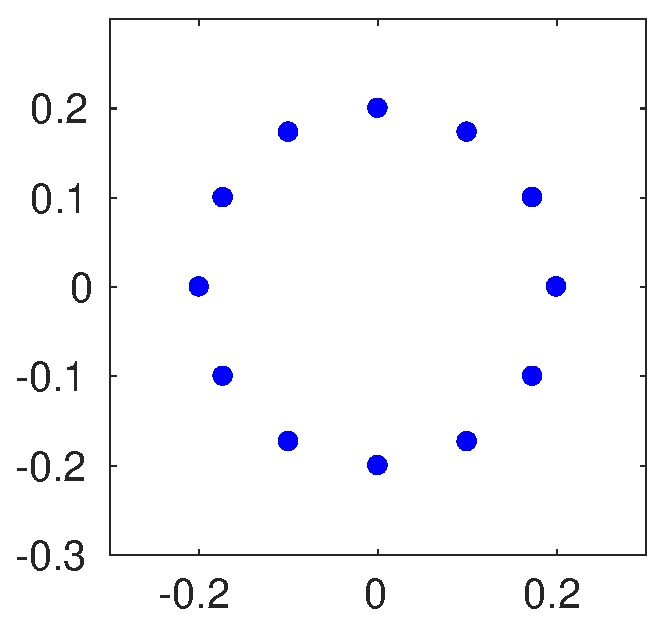
\includegraphics[height=0.24\textwidth]{figs/fig_guideExpSetupTrans}
  }
\end{subcaptionbox}
\begin{subcaptionbox}{Transmitters in 3D.
   \label{fig:guide:expSetupTrans3D}}[0.28\textwidth]{
   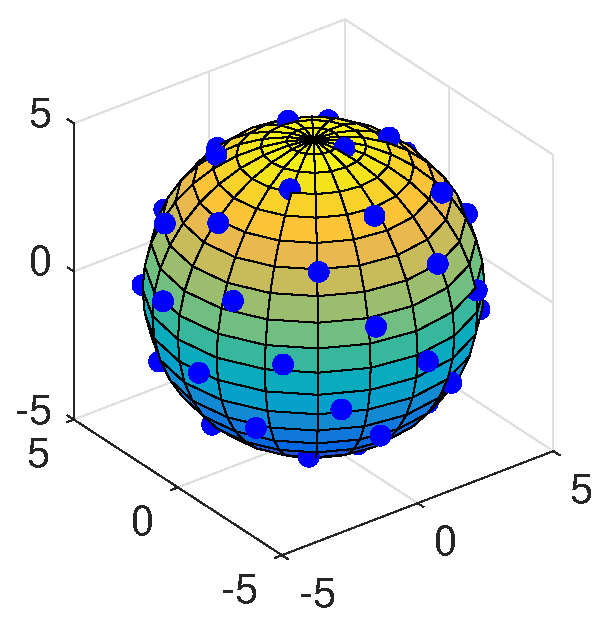
\includegraphics[height=0.24\textwidth]{figs/fig_guideExpSetupTrans3D}
  }
\end{subcaptionbox}
\begin{subcaptionbox}{Receivers.
   \label{fig:guide:expSetupRece}}[0.28\textwidth]{
   \includegraphics[height=0.24\textwidth]{figs/fig_guideExpSetupRece}
  }
\end{subcaptionbox}
\caption{\subref{fig:guide:expSetupTrans}~Transmitters on a circle as generated by Lst.~\ref{lst:guideExpSetupTrans}. 
\subref{fig:guide:expSetupTrans3D}~Transmitters on a sphere as generated by Lst.~\ref{lst:guideExpSetupTrans3D}. 
\subref{fig:guide:expSetupRece}~Receivers on a square as generated by Lst.~\ref{lst:guideExpSetupRece}.}
\label{fig:guide:expSetupTransAndRecei}
\end{figure}

\paragraph{Transmitters' Positions} The geometric shape of the transmitters can be generated by the function \textsf{setIncPnts}. 
%
It requires the dimension by $d = \textsf{seti.dim}$ (2 or 3) and the type of the incident field by \textsf{seti.incType} (\textsf{'pointSource'} or \textsf{'planeWave'}). The other input arguments depend on the shape chosen by \textsf{seti.incPntsType}. The user is also free to define his own positions. Further details are given in~\textsf{setIncPnts.m} and~\textsf{pntsGeometry.m}.
%
Note that plane waves only depend on direction, such that the radius \textsf{seti.radSrc} is set to 1 in this case.
%
The output arguments are the coordinates of the transmitters stored in \textsf{seti.incPnts} as a real matrix of size $d \times N_\Inc$, the number of transmitters $N_\Inc = \textsf{seti.incNb}$ and the approximation of the infinitesimal element of closed contour with control points stored in \textsf{seti.dSInc}. (If a closed contour does not make sense, it is set to $1$.)

Lst.~\ref{lst:guideExpSetupTrans} arranges 12 transmitters emitting point sources on a circle with radius~$0.2$ and results in Fig.~\ref{fig:guide:expSetupTrans}.
\begin{lstlisting}[caption={Arrange transmitters on a circle (\emph{source code}: \textsf{guides/guideExpSetupTrans.m}).},label=lst:guideExpSetupTrans]
init; seti.dim = 2;
seti.incType = 'pointSource';
seti.incPntsType = 'circle'; seti.radSrc = 0.2; seti.incNb = 12;
seti = setIncPnts(seti);
plot(seti.incPnts(1,:),seti.incPnts(2,:),'b.');
\end{lstlisting}

Lst.~\ref{lst:guideExpSetupTrans3D} arranges 49 transmitters emitting point sources on a sphere with radius~$5$ and results in Fig.~\ref{fig:guide:expSetupTrans3D}. Note that in fact 49 transmitters are arranged because 50 is an even number. 
\begin{lstlisting}[caption={Arrange transmitters on a sphere (\emph{source code}: \textsf{guides/guideExpSetupTrans3D.m}).},label=lst:guideExpSetupTrans3D]
init; seti.dim = 3;
seti.incType = 'pointSource';
seti.incPntsType = 'sphereFibo'; seti.radSrc = 5; seti.incNb = 50;
seti = setIncPnts(seti);
[sx,sy,sz] = sphere; r = seti.radSrc; surf(sx*r,sy*r,sz*r); hold on;
Pnts = seti.incPnts; s = 100; scatter3(Pnts(1,:),Pnts(2,:),Pnts(3,:),s,'filled','b'); hold off;
\end{lstlisting}

\paragraph{Receivers' Positions} The same geometric shapes available for transmitters are also available for receivers. Therefore the function \textsf{setMeasPnts} is the analogy of \textsf{setIncPnts}. 
%
The main difference is the choice of the type of the measured field (instead of the incident field) by \textsf{seti.measType} (\textsf{'nearField'} or \textsf{'farField'}). The shape is chosen by \textsf{seti.measPntsType}, see~\textsf{setMeasPnts.m} and~\textsf{pntsGeometry.m} for details.
%
The output arguments are analogous to the function \textsf{setIncPnts}, i.e. the coordinates are stored in \textsf{seti.measPnts}, the number in \textsf{seti.measNb} and the infinitesimal element in \textsf{seti.dSMeas}.
%
We stress that a far field only depends on the direction. Therefore \IPscatt chooses \textsf{seti.measPnts} as a circle (or a sphere) of radius one in this case and uses these points as argument for the computed far field.

Lst.~\ref{lst:guideExpSetupRece} arranges $4+1$ points on each edge of a square with length~$0.8$ and resulting receivers are plotted in Fig.~\ref{fig:guide:expSetupRece}.

\begin{lstlisting}[caption={Arrange receivers on a square (\emph{source code}: \textsf{guides/guideExpSetupRece.m}).},label=lst:guideExpSetupRece]
init; seti.dim = 2;
seti.measType = 'nearField';
seti.measPntsType = 'square'; seti.measNbEdge = 4; seti.measEdgeLength = 0.8;
seti = setMeasPnts(seti);
plot(seti.measPnts(1,:),seti.measPnts(2,:),'rs');
\end{lstlisting}

\paragraph{Incident Field} The routine \textsf{seti = setIncField(seti)} evaluates the incident fields on the region of interest (ROI) for each transmitter and stores them in \textsf{seti.incField}.

\paragraph{Details of \textsf{setIncField}} Remember that the incident field $u^\Inc$ solves the Helm\-holtz equation, see~\eqref{eq:HEQinc}. Typical choices of $u^\Inc$ include plane waves and point sources and are provided by \IPscatt. 

Let $u_\mathrm{plane}^\Inc(x) = \exp(\im k \langle x, \theta \rangle)$ be the incident field at position $x$ in the case of a \emph{plane wave} (in 2D and 3D) where $\theta$ is the direction. Then the incident fields of $N_\Inc$ plane waves with directions $\theta_j$, $j = 1,\ldots,N_\Inc$, at points $x$ in ROI are stored as a complex matrix $\texttt{seti.incField} = (\exp(\im k \langle x, \theta_j \rangle))$ of size $\NROI \times N_\Inc$.

In the case of a \emph{point source} at transmitter position~$y$ the incident field is defined by $u_\mathrm{point}^\mathrm{i}(x) = \Phi(x-y)$ for points $x$ in ROI, where $\Phi$ is radiating fundamental solution, see~\eqref{eq:fundamental}, of the Helmholtz equation. The incident fields at points $x$ in ROI of $N_\Inc$ point sources at positions $y_j$, $j = 1, \ldots, N_\Inc$, are stored as a complex matrix $\texttt{seti.incField} = (\Phi(x-y_j))$ again of size $\NROI \times N_\Inc$.

For further information concerning incident fields see~\cite[Ch. 3.5 and 8.4]{Colton2013} or~\cite[Sec.~3.5]{Buergel2017}.

\paragraph{Input Arguments of \textsf{setIncField}} The routine \textsf{setIncField} requires the already introduced number of transmitters \textsf{seti.incNb}, their positions \textsf{seti.incPnts} and the grid-related arguments \textsf{seti.nROI} and \textsf{seti.gridROI}. Furthermore, the following arguments are needed:

\noindent\begin{tabular}[t]{p{2cm} p{13.6cm}}
\textsf{seti.incType} & Type of the incident field (\textsf{'pointSource'} or \textsf{'planeWave'}).\\
\textsf{seti.k}       & Wave number (in reciprocal meters).\\
\textsf{seti.model}   & Chosen model of the problem (\textsf{'helmholtz2D'} or \textsf{'helmholtz3D'}).
\end{tabular}

\paragraph{Output Argument of \textsf{setIncField}} The incident field in the region of interest for each transmitter is stored in \textsf{seti.incField} as a complex matrix of size $\NROI \times N_\Inc$. Note that ROI is stored as a vector of size $\NROI$ (remember that $\NROI = \textsf{seti.nROI}^d$ with $d = \textsf{seti.dim}$) instead of a matrix to use a matrix multiplication when evaluating the forward operator, cf.~\eqref{eq:forward}. The number of incident fields is $N_\Inc = \texttt{seti.incNb}$.

\paragraph{Measurement Kernel} The measurement kernel \textsf{seti.measKer} is computed in \textsf{setMeasKer} for each receiver. It is needed to evaluate the sensor measurements $u^\Sca|_\RXM = k^2 \kappa\, q \pmul u^\Tot \mathcal{V}$ at the receivers' positions $\RXM$ for near field data, i.e. to evaluate the forward operator for one incident field, cf.~\eqref{eq:simo} and~\eqref{eq:forwardCodeSingle}. The used quantities are the wave number $k = \textsf{seti.k}$, the measurement kernel $\kappa = \textsf{seti.measKer}$, the contrast $q = \textsf{seti.qROI}$, the total field $u^\Tot = u^\Inc+u^\Sca = \textsf{uIncROI+uScattROI}$ and the voxel volume $\mathcal{V} = \textsf{seti.dV}$. The notation $f \pmul g$ stresses the pointwise multiplication in the discretized case. The above formula also evaluates sensor measurements at the directions in $\RXM$ in the case of far field data, cf.~\eqref{eq:solToDataFar} for the differing measurement kernel.

\paragraph{Input Arguments of \textsf{setMeasKer}} The input arguments of \textsf{setMeasKer} are almost the same as in \textsf{setIncField}. The only difference is that \textsf{seti.incType}, \textsf{seti.incNb} and \textsf{seti.incPnts} are replaced by \textsf{seti.measType} to set the type of the scattered field (\textsf{'nearField'} or \textsf{'farField'}), $N_\Sca = \textsf{seti.measNb}$ for the number of receivers and \textsf{seti.measPnts} to set the coordinates of the receivers (real matrix of size $d \times N_\Sca$ with $d = \textsf{seti.dim}$).

\paragraph{Output Argument of \textsf{setMeasKer}} The measurement kernel in ROI for each receiver is stored in \textsf{seti.measKer} (complex matrix of size $N_\Sca \times \NROI$).

\paragraph{Example for the Incident Field and the Measurement Kernel} Lst.~\ref{lst:guideExpSetup} demonstrates the use of \textsf{setIncField} and \textsf{setMeasKer} following Lst.~\ref{lst:guideSetGrid},~\ref{lst:guideExpSetupTrans} and~\ref{lst:guideExpSetupRece}. The resulting fields are visualized in Fig.~\ref{fig:guide:expSetup}.

\begin{lstlisting}[caption={Incident field (\textsf{setIncField}) and measurement kernel (\textsf{setMeasKer}) (\emph{source code}: \textsf{guides/guideExpSetup.m}).},label=lst:guideExpSetup]
init;
guideExpSetupTrans; guideExpSetupRece; guideSetGrid;
seti.model = 'helmholtz2D'; 
seti.k = 250;
seti = setIncField(seti); 
seti = setMeasKer(seti);
figure(1); imagesc(real(reshape(seti.incField(:,1),[seti.nROI seti.nROI]))); axis xy; colorbar;
figure(2); imagesc(real(reshape(seti.measKer(5,:),[seti.nROI seti.nROI]))); axis xy; colorbar;
\end{lstlisting}

\begin{figure}
\centering
\begin{subcaptionbox}{Incident field.
   \label{fig:guide:expSetup1}}[0.28\textwidth]{
   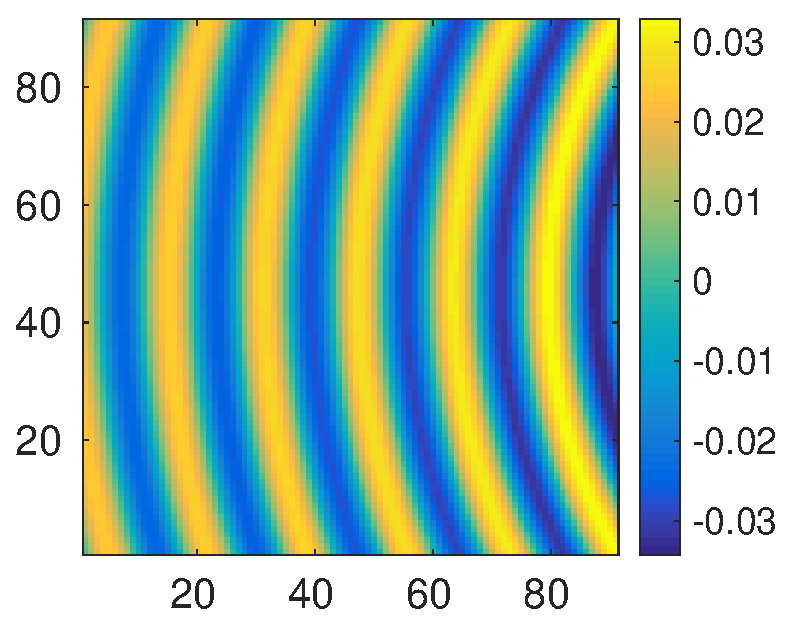
\includegraphics[height=0.24\textwidth]{figs/fig_guideExpSetup1}
  }
\end{subcaptionbox}\hspace{2em}
\begin{subcaptionbox}{Measurement kernel.
   \label{fig:guide:expSetup2}}[0.28\textwidth]{
   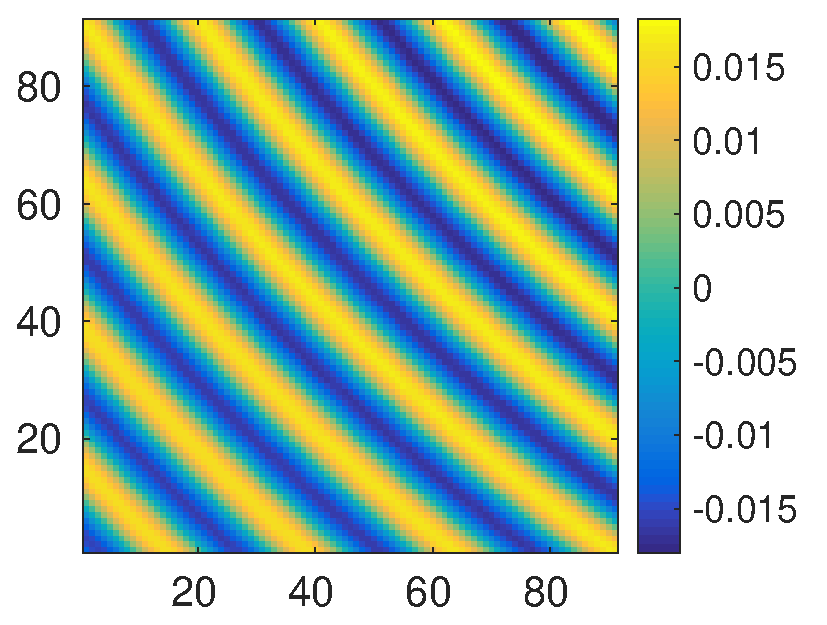
\includegraphics[height=0.24\textwidth]{figs/fig_guideExpSetup2}
  }
\end{subcaptionbox}
\caption{Evaluated fields in the region of interest as generated by Lst.~\ref{lst:guideExpSetup}.
\subref{fig:guide:expSetup1}~Real part of the incident field of the \nth{1} transmitter. 
\subref{fig:guide:expSetup2}~Real part of the measurement kernel of the \nth{5} receiver. 
}
\label{fig:guide:expSetup}
\end{figure}

%%

\subsection{Guide: Defining a Contrast}\label{sec:guide:contrast}

The functions generating the predefined contrasts are stored in the subfolders of the directory \textsf{incontrasts}. In 2D e.g. a corner, a cross, a ball and a combination of two corners and one ball are provided. Also, a contrast with one dielectric cylinder and another contrast with two dielectric cylinders as considered in the experiments from Institute Fresnel are available. In 3D \IPscatt provides a tripod, a cross, a ball and the edges of a cube. For a full list see~\textsf{incontrastsRef.m}. 
To build own contrasts the user can create new files in the directory \textsf{incontrasts} (or its subfolders)---analogously to existing functions.

\paragraph{Input Arguments} The input arguments are two or three coordinate arrays (depending on the dimension) and the structure array \textsf{seti}. The coordinate arrays are vectors with the size of the region of interest, i.e. $1 \times \textsf{seti.nROI}^d$ with $d = \textsf{seti.dim}$, see \textsf{setGrid} in Sec.~\ref{sec:guide:setGrid}. The structure array \textsf{seti} is an input argument to scale the size of the contrast by \textsf{seti.rCD} (as defined in \textsf{setGrid}). Further, some contrasts require additional input, e.g. for balls one needs to set the contrast value \textsf{seti.qBall} and the radius \textsf{seti.rBall}.

\paragraph{Output Argument} The output argument is the contrast $\textsf{q}$ stored as a vector, i.e. of size $1 \times \textsf{seti.nROI}^d$ with $d = \textsf{seti.dim}$.

\paragraph{Example} In Lst.~\ref{lst:guideContrast} we consider a ball of radius 0.05 and contrast value 0.8 in two and three dimensions. The results are shown in Fig.~\ref{fig:guide:contrast}. Note that the file \textsf{guideSetGrid3D} contains the same code as \textsf{guideSetGrid} apart from \textsf{seti.dim = 3} instead of \textsf{seti.dim = 2}. Further, note that \IPscatt provides the convenience function \textsf{contourPlotROI} to plot the surface of 3D objects.

\begin{lstlisting}[caption={Predefined contrasts in 2D and 3D (\emph{source code}: \textsf{guides/guideContrast.m}).},label=lst:guideContrast]
init; seti.rBall = 0.05; seti.qBall = 0.8;
%
guideSetGrid;
q2D = referenceBall2D(seti.gridROI(1,:), seti.gridROI(2,:), seti);
x = seti.gridROI(1,:); y = seti.gridROI(2,:);
figure(1); imagesc(x,y,real(reshape(q2D,[seti.nROI seti.nROI]))); axis xy; colorbar;
%
guideSetGrid3D;
q3D = referenceBall3D(seti.gridROI(1,:), seti.gridROI(2,:), seti.gridROI(3,:), seti);
figure(2); contourPlotROI(q3D, seti, 'real');
\end{lstlisting}

\begin{figure}
\centering
\begin{subcaptionbox}{Ball in 2D.
  \label{fig:contrast:2D}}[0.31\textwidth]{
  \includegraphics[height=0.24\textwidth]{figs/fig_guideContrast2D}
  }
\end{subcaptionbox}
\begin{subcaptionbox}{Ball in 3D.
  \label{fig:contrast:3D}}[0.31\textwidth]{
  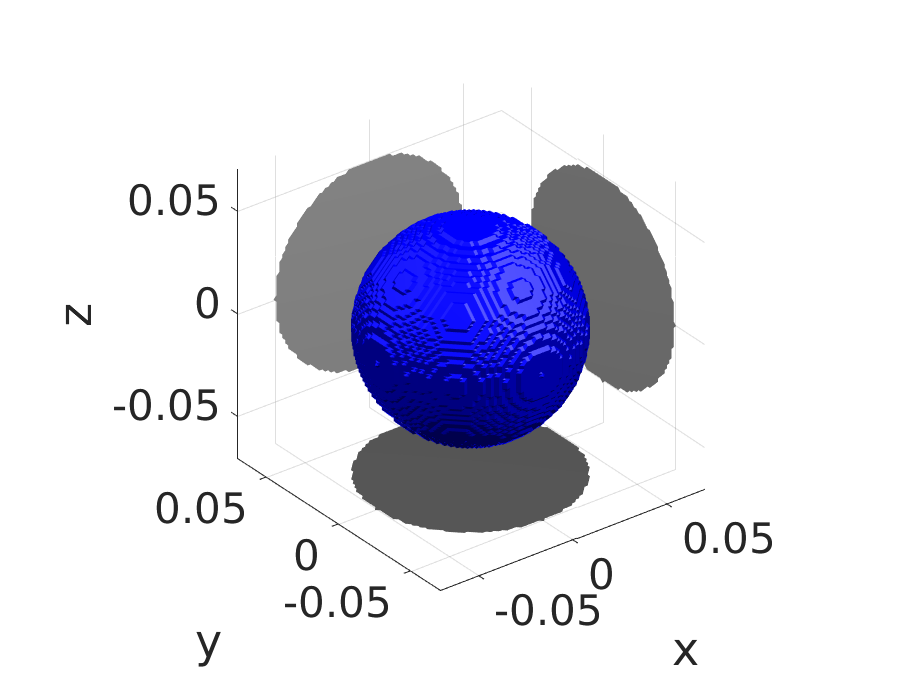
\includegraphics[height=0.26\textwidth]{figs/fig_guideContrast3D}
  }
\end{subcaptionbox}
\caption{Predefined contrasts in 2D and 3D as generated by Lst.~\ref{lst:guideContrast}.}
\label{fig:guide:contrast}
\end{figure}

%%

\subsection{Guide: Setting up Geometry and Simulation}\label{sec:guide:setGeomSim}

As already mentioned \IPscatt takes care that all necessary fields of the structure array \textsf{seti} are set in a consistent manner. The routine \textsf{setGeomSim} does this for the grid, the experimental set-up (transmitters' and receivers' positions, incident field and measurement kernel) and the contrast as described in Sec.~\ref{sec:guide:setGrid}, \ref{sec:guide:expSetup} and~\ref{sec:guide:contrast}.

\paragraph{Input Arguments} The input arguments are the fields of the structure array \textsf{seti} as described in the input and output arguments in the just-mentioned sections. In comparison to Lst.~\ref{lst:guideContrast} the routine expects the function's name of the chosen contrast as string stored in \textsf{seti.contrast}. Further, in the case of two dimensions \textsf{seti.rotation} contains the number of degrees (default: 0) by which the contrast is rotated in the mathematically positive sense. Empty fields are set to default values.

\paragraph{Output Arguments} The essential fields of the output argument \textsf{seti} were already described in the aforementioned sections except for the contrast (evaluated on the region of interest) which is saved in \textsf{seti.qROIexact} as a vector of size $\textsf{seti.nROI}^d \times 1$ with $d = \textsf{seti.dim}$, see \textsf{setGrid} in Sec.~\ref{sec:guide:setGrid}.

\paragraph{Example} As before we consider a circle as contrast with radius $0.05$ and contrast value $0.8$. The experimental set-up is not defined explicitly such that default values are used in Lst.~\ref{lst:guideSetGeomSim}. 
Note that \textsf{seti.G} as used in Lst.~\ref{lst:guideSetGeomSim} is a convenience function (defined in \textsf{setGeomSim}) to avoid \textsf{reshape}. 
For the demonstration of the rotation we refer to Lst.~\ref{lst:guideForward}. 

\begin{lstlisting}[caption={Set the experimental set-up and the contrast by \textsf{setGeomSim} (\emph{source code}: \textsf{guides/guideSetGeomSim.m}).},label=lst:guideSetGeomSim]
init; seti.rBall = 0.05; seti.qBall = 0.8; 
seti.contrast = 'referenceBall2D';
seti = setGeomSim(seti);
imagesc(real(seti.G(seti.qROIexact))); axis xy; colorbar;
\end{lstlisting}

The routine \textsf{setGeomSim} can be used to set the optional input argument \textsf{dispDepth}. This argument controls the depth of displayed messages, that is demonstrated in Lst.~\ref{lst:guideSetGeomSimDisp}. For more information see Sec.~\ref{sec:guide:convenience}.

\begin{lstlisting}[caption={Routine \textsf{setGeomSim} with optional input argument \textsf{dispDepth} (\emph{source code}: \textsf{guides/guideSetGeomSimDisp.m}).},label=lst:guideSetGeomSimDisp]
init; clear seti; seti = struct; seti = setGeomSim(seti,1);
\end{lstlisting}

%%

\subsection{Guide: Evaluating the Forward Operator}\label{sec:guide:forward}

With the defined grid, experimental set-up and contrast we can compute the scattered field at the receivers' positions with the forward operator $\F$ (multi-static contrast-to-measurement operator), see~\eqref{eq:forward}. This is done by means of the routine \textsf{forward}. The reader should keep in mind that the receivers measure the total field, in particular when considering real-world data from Institute Fresnel. However, \IPscatt directly provides the scattered field, i.e. the difference between the total and incident field.

\paragraph{Input Arguments} The routine \textsf{forward} requires the grid, the experimental set-up and the contrast as preparations. Therefore the structure array \textsf{seti} is required as described in Sec.~\ref{sec:guide:setGrid}, \ref{sec:guide:expSetup} and~\ref{sec:guide:contrast}. It is recommended to use \textsf{setGeomSim} to set all necessary fields of the structure array \textsf{seti} in a consistent manner, see Sec.~\ref{sec:guide:setGeomSim}. Further, the routine requires the contrast \textsf{qROI} (complex matrix stored as a vector of size $\textsf{seti.nROI}^d \times 1$ with $d = \textsf{seti.dim}$, see \textsf{setGrid} in Sec.~\ref{sec:guide:setGrid}).

\paragraph{Output Arguments} \hfill

\noindent\begin{tabular}[t]{p{1.5cm} p{14.1cm}}
\textsf{FFqMeas} & The field~\textsf{FFqMeas} contains the data, i.e. the result of the forward operator $\F$ evaluated on the underlying contrast $q$, see~\eqref{eq:forwardCode}. This result is the scattered field evaluated on receivers' positions for each transmitter. Therefore \textsf{FFqMeas} is a complex matrix of size $\textsf{seti.measNb} \times \textsf{seti.incNb}$.\\
\textsf{FFqROI}  & The field~\textsf{FFqROI} stores the scattered field evaluated on the region of interest (ROI) for each of the $N_\Inc$ transmitters, see~\eqref{eq:FFqROI}. Therefore \textsf{FFqROI} is a complex matrix of size $\textsf{seti.nROI}^d \times N_\Inc$ with $d = \textsf{seti.dim}$ and $N_\Inc = \textsf{seti.incNb}$.\\
\textsf{seti}    & The structure array~\textsf{seti} contains the settings used for generating the other outputs. We stress that \textsf{forward()} sets all fields to default values. In this case these settings are interesting.
\end{tabular}

\paragraph{Example} Lst.~\ref{lst:guideForward} evaluates and visualizes the scattered field in the region of interest and at the receivers' positions for each transmitter. The underlying contrast is a corner plotted with the results in Fig.~\ref{fig:guide:forward}. 
For more information see~\textsf{forward.m} and~\textsf{mimo.m}.

\begin{lstlisting}[caption={Compute the scattered field by the routine \textsf{forward} for a corner-shaped contrast rotated by $20^\circ$ (\emph{source code}: \textsf{guides/guideForward.m}).},label=lst:guideForward]
init; seti.contrast = 'corner2D'; seti.rotation = 20;
seti = setGeomSim(seti);
figure(1); imagesc(real(seti.G(seti.qROIexact))); axis xy; colorbar;
[FFqMeas,FFqROI,seti] = forward(seti,seti.qROIexact);
figure(2); imagesc(real(seti.G(FFqROI(:,7)))); axis xy; colorbar; % 7th transmitter
figure(3); imagesc(real(FFqMeas)); axis xy; colorbar;
\end{lstlisting}

\begin{figure}
\centering
\begin{subcaptionbox}{Predefined contrast.
  \label{fig:guide:forward1}}[0.31\textwidth]{
  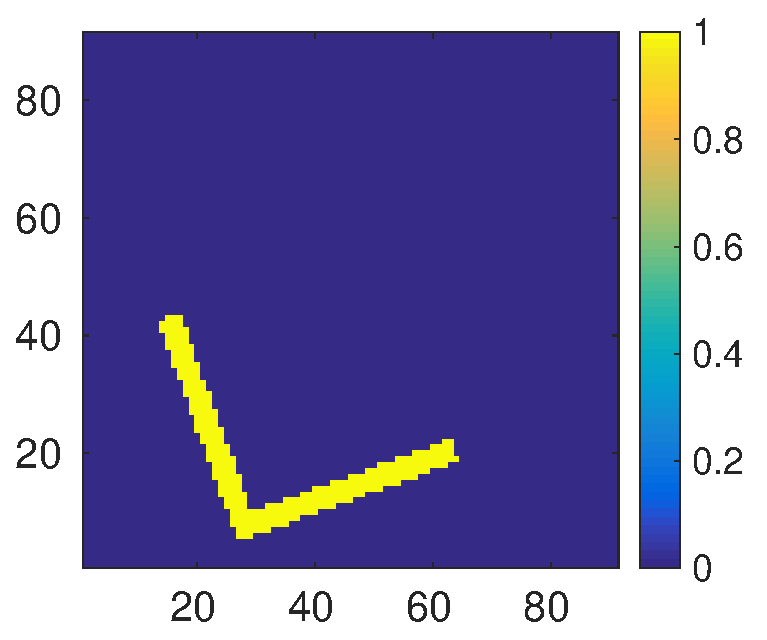
\includegraphics[height=0.21\textwidth]{figs/fig_guideForward1}
  }
\end{subcaptionbox}
\begin{subcaptionbox}{Data.
  \label{fig:guide:forward2}}[0.31\textwidth]{
  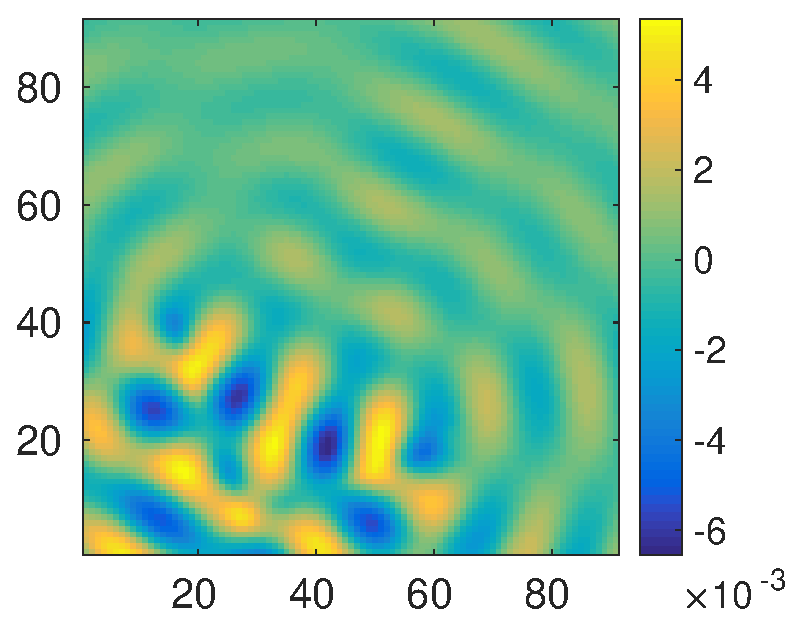
\includegraphics[height=0.21\textwidth]{figs/fig_guideForward2}
  }
\end{subcaptionbox}
\begin{subcaptionbox}{Scattered field.
  \label{fig:guide:forward3}}[0.31\textwidth]{
  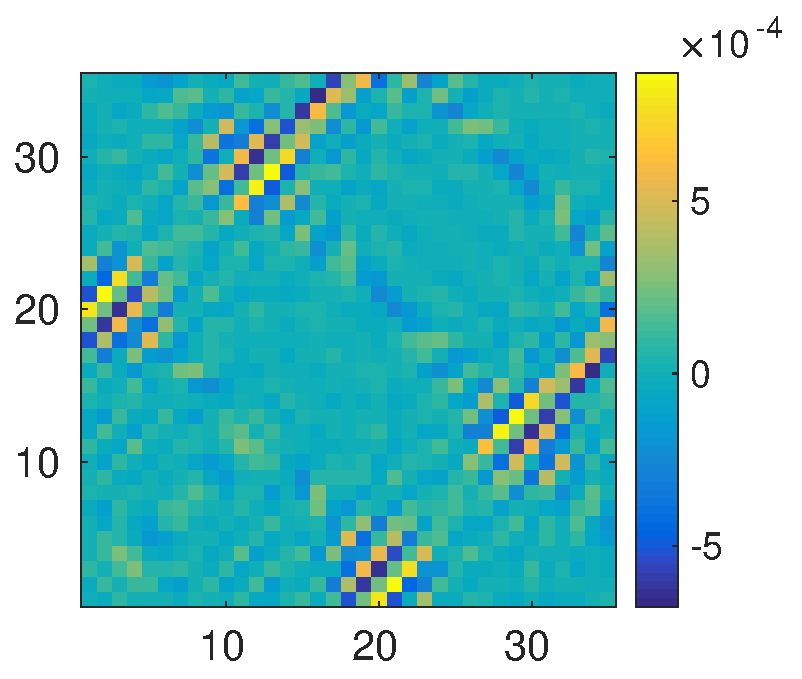
\includegraphics[height=0.23\textwidth]{figs/fig_guideForward3}
  }
\end{subcaptionbox}
\caption{The results generated by Lst.~\ref{lst:guideForward}. 
\subref{fig:guide:forward1}~The contrast \textsf{corner2D} rotated by $20^\circ$. \subref{fig:guide:forward2}~The resulting scattered field in the region of interest for the \nth{7} transmitter. 
\subref{fig:guide:forward3}~The scattered field at the receivers' positions for each transmitter. (The experimental set-up consists of 35~transmitters and 35~receivers equidistantly arranged on a circle.)}
\label{fig:guide:forward}
\end{figure}

%%

\subsection{Guide: Evaluating the Fr\'echet Derivative (Jacobian Matrix)}\label{sec:guide:derivative}

In finite-dimensional spaces the Fr\'{e}chet derivative~$\F'(q)[h]$ of the forward operator~$\F$ at the contrast~$q$ evaluated on~$h$, see~\eqref{eq:DFFqc}, is represented by the Jacobian matrix evaluated on~$h$. This matrix is required in the variational reconstruction, see Sec.~\ref{sec:guide:recon}, and evaluated by the routine \textsf{derivative}.
%
Therefore the routine \textsf{derivative} provides auxiliary matrices \textsf{JA} and \textsf{JB} which are necessary for the Jacobian matrix of $\F$ at the contrast $q$. These matrices can be used to construct~$\F'(q)[h]$ via \textsf{JA*diag(h)*JB}. The corresponding function handle is denoted by~\textsf{DFFq} in the code snippet. The result is a complex matrix of size $\textsf{seti.measNb} \times \textsf{seti.incNb}$.

\paragraph{Input Arguments} As the routine \textsf{derivative} requires the grid, the experimental set-up and the contrast as preparations, it is recommended to use \textsf{setGeomSim} to set all necessary fields of the structure array \textsf{seti} in a consistent manner, see Sec.~\ref{sec:guide:setGeomSim} and Lst.~\ref{lst:guideSetGeomSim}. Apart from that, the contrast $q = \textsf{qROI}$ in the region of interest (complex matrix as vector of size $\textsf{seti.nROI}^d \times 1$ with $d = \textsf{seti.dim}$) is an input argument.

\paragraph{Output Arguments} The auxiliary matrices \textsf{JA} and \textsf{JB} are the output arguments, see~\eqref{eq:DFFqd}. (These are complex matrices of size $\textsf{seti.measNb} \times \NROI$ and $\NROI \times \textsf{seti.incNb}$ with $\NROI = \textsf{seti.nROI}^d$ and $d = \textsf{seti.dim}$.)

\paragraph{Example} Lst.~\ref{lst:guideDerivative} shows how to evaluate $\F'(q)[h]$. We have chosen a corner-shaped contrast rotated by $20^\circ$, see Fig.~\ref{fig:guide:forward1}, and for the sake of simplicity a constant update $h = 1 + \im$. The result is plotted in Fig.~\ref{fig:guide:derivative}. 
For more information see~\textsf{derivative.m} and~\textsf{mimo.m}. 

\begin{lstlisting}[caption={Compute the Fr\'{e}chet derivative {$\F'(q)[h]$} (\emph{source code}: \textsf{guides/guideDerivative.m}).},label=lst:guideDerivative]
init; seti.contrast = 'corner2D'; seti.rotation = 20;
seti = setGeomSim(seti);
qROI = seti.qROIexact;
[JA,JB] = derivative(seti,qROI);
%
DFFq = @(h) JA*diag(h)*JB;
h = ones(size(qROI))+1i*ones(size(qROI));
DFFqh = DFFq(h);
imagesc(real(DFFqh)); axis xy; colorbar;
\end{lstlisting}

\begin{figure}
\centering
\begin{subcaptionbox}{Derivative.
  \label{fig:guide:derivative}}[0.28\textwidth]{
  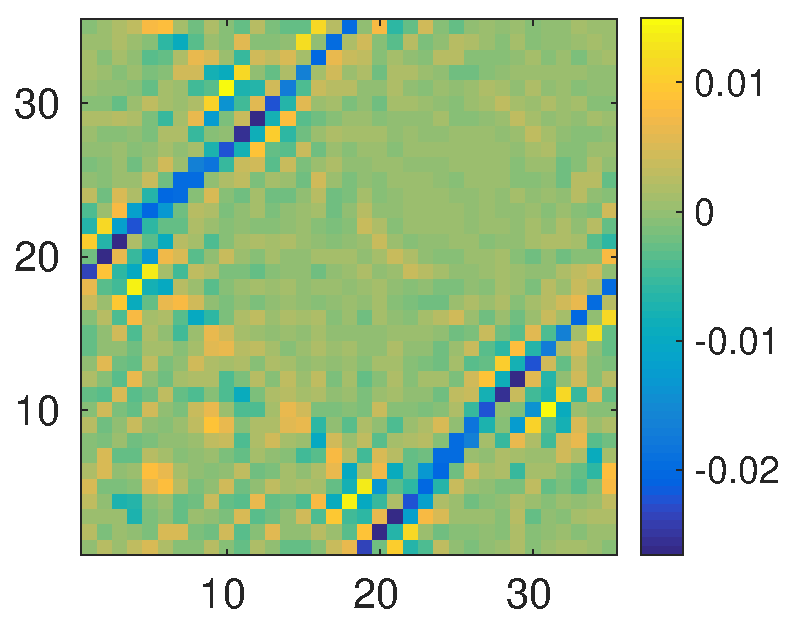
\includegraphics[height=0.22\textwidth]{figs/fig_guideDerivative}
  }
\end{subcaptionbox}
\begin{subcaptionbox}{Adjoint of the derivative at the defect.
  \label{fig:guide:adjOfDer}}[0.28\textwidth]{
   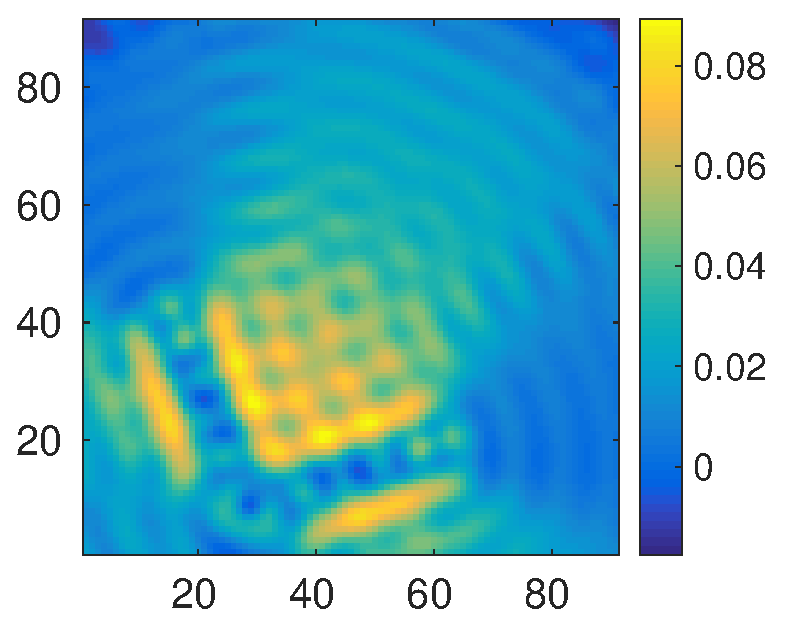
\includegraphics[height=0.22\textwidth]{figs/fig_guideAdjOfDer}
  }
\end{subcaptionbox}
\caption{\subref{fig:guide:derivative}~The Fr\'{e}chet derivative $\F'(q)[h]$ as generated by Lst.~\ref{lst:guideDerivative}. 
\subref{fig:guide:adjOfDer}~The adjoint of the derivative at the defect as generated by Lst.~\ref{lst:guideAdjOfDer}.}
\label{fig:guide:derivativeAndAdjOfDer}
\end{figure}

%%

\subsection{Guide: Evaluating the Adjoint of the Derivative at the Defect}\label{sec:guide:adjOfDer}

\IPscatt can evaluate the adjoint of the derivative of the forward operator applied to the defect $\F(q) - \msdata^\delta$ by the routine \textsf{adjOfDer}. That is, it computes $\textsf{ADFFq} = [\F'(q)]^\ast [\F(q) - \msdata^\delta]$, which is the derivative of the least-squares error of the forward operator, see~\eqref{eq:ADFFqc}. For the forward operator $\F$, see~\eqref{eq:forward} and Sec.~\ref{sec:guide:forward}, for the contrast $q = \textsf{qROI}$, see Sec.~\ref{sec:guide:contrast}, and for the data $\msdata^\delta$ with noise level $\delta$, see Sec.~\ref{sec:guide:addNoise}.
%
Although the routine \textsf{adjOfDer} is not part of our reconstruction scheme, we provide it, because it is an important ingredient of many other reconstruction schemes, e.g. the thresholded, nonlinear Landweber based on the so-called soft-shrinkage operator, see~\cite{Chan2005}. 

\paragraph{Input Arguments} The function \textsf{adjOfDer} requires the grid, the experimental set-up and the contrast. The routine \textsf{setGeomSim} is recommended to set all necessary fields of the structure array \textsf{seti} in a consistent manner, see Sec.~\ref{sec:guide:setGeomSim}. Further, the contrast \textsf{qROI} in the region of interest (complex matrix stored as vector of size $\textsf{seti.nROI}^d \times 1$ with dimension $d = \textsf{seti.dim}$) and the data $\textsf{FmeasDelta} = \msdata^\delta$ at receivers' positions (matrix of size $\textsf{seti.measNb} \times \textsf{seti.incNb}$) are required.

\paragraph{Output Arguments} The output arguments are the adjoint of the derivative applied to the defect, \textsf{ADFFq} (complex matrix stored as vector of size $\textsf{seti.nROI}^d \times 1$ with $d = \textsf{seti.dim}$), and the structure array \textsf{seti} containing all parameters of the setting. This structure array is interesting if all or some fields were set automatically.

\paragraph{Example} Lst.~\ref{lst:guideAdjOfDer} contains the code to compute the adjoint of the derivative applied to the defect $\textsf{FFqmF} = \F(q) - \msdata^\delta$, where $q = \textsf{qROI}$ is the contrast from Fig.~\ref{fig:guide:forward1}. In this simple example the data \textsf{FmeasDelta} is set to zero. The result is shown in Fig.~\ref{fig:guide:adjOfDer}.

\begin{lstlisting}[caption={Compute the adjoint of the derivative at the defect (\emph{source code}: \textsf{guides/guideAdjOfDer.m}).},label=lst:guideAdjOfDer]
init; seti.contrast = 'corner2D'; seti.rotation = 20;
seti = setGeomSim(seti);
qROI = seti.qROIexact;
FmeasDelta = zeros(seti.measNb,seti.incNb);
[ADFFq,seti] = adjOfDer(seti,qROI,FmeasDelta);
imagesc(real(seti.G(ADFFq))); axis xy; colorbar;
\end{lstlisting}

Note that it is possible to evaluate the defect~$\textsf{FFqmF}$ as well as the adjoint of the derivative at the defect, \textsf{ADFFq}, in a single function call by \textsf{[FFqmF,ADFFq] = mimo(seti,qROI,FmeasDelta,'adjOfDer')}, see~\textsf{adjOfDer.m} and~\textsf{mimo.m} for more information.

%%

\subsection{Guide: Generating Simulated Data with Noise}\label{sec:guide:addNoise}

\IPscatt provides the option to add a specific relative noise level $\delta > 0$ to the exact data $\msdata = \F(q)$ for the contrast $q$ as in Sec.~\ref{sec:guide:forward}. This results in perturbed data
\[
\msdata^\delta = \msdata + \delta\, \frac{N_\real + \im N_\imag}{\|N_\real + \im N_\imag\|_\fro} \|\msdata\|_\fro,
\]
where $N_{\mathrm{Re}},N_{\mathrm{Im}} \in \R^{N_\Sca \times N_\Inc}$ are two real matrices with normally distributed entries ($N_\Sca = \texttt{seti.measNb}$ is the number of receivers and $N_\Inc = \texttt{seti.incNb}$ the number of transmitters) and Frobenius norm $\|\cdot\|_\fro$. The corresponding function to add noise is called \textsf{addNoise}.

\paragraph{Input Arguments} Input arguments of \textsf{addNoise} are the structure array \textsf{seti} with the infinitesimal element \textsf{seti.dSMeas}, see Sec.~\ref{sec:guide:expSetup}, and the exact data $\textsf{FmeasExact} = \F(q)$, that was defined as \textsf{FFqMeas} in Sec.~\ref{sec:guide:forward}. The following fields of \textsf{seti} are set to default values if they are not defined.

\noindent\begin{tabular}[t]{p{2.2cm} p{13.4cm}}
\textsf{seti.delta} 	 & Relative (artificial) noise level $\delta$ of the data (default: 0.01).\\
\textsf{seti.whichNoise} & The following values are used to choose the type of the propability density function to perturb the data: \textsf{'laplace'}, \textsf{'uniform'}, \textsf{'normal'} (default). By default the mean value of all densities vanishes.\\
\textsf{seti.seed} 	 & Non-negative integer (default: 0) to control the random number generator.
\end{tabular}

\paragraph{Output Arguments} The structure array \textsf{seti} contains the used settings. Therefore it is only interesting as an output argument if the optional fields \textsf{delta}, \textsf{whichNoise} or \textsf{seed} were set automatically. The output argument $\textsf{FmeasDelta} = \msdata^\delta$ contains the perturbed data (a complex matrix of size $\textsf{seti.measNb} \times \textsf{seti.incNb}$).

\paragraph{Example} In Lst.~\ref{lst:guideAddNoise} the number of 10~receivers and 5~transmitters was used. The infinitesimal element of the receivers was set to be~1 by \textsf{seti.dSMeas = 1}. Furthermore, a matrix with random entries is used as exact data. This data is perturbed by a normally distributed noise with a relative noise level of $5\%$. The result is stored in \textsf{FmeasDelta}.

\begin{lstlisting}[caption={Adding noise to exact data (\emph{source code}: \textsf{guides/guideAddNoise.m}).},label=lst:guideAddNoise]
init; FmeasExact = rand(10,5) + 1i*rand(10,5); seti.dSMeas = 1;
seti.delta = 0.05; seti.whichNoise = 'normal'; seti.seed = 10;
[seti, FmeasDelta] = addNoise(seti, FmeasExact);
\end{lstlisting}

\paragraph{Example of Convenience Function \textsf{setData}} The convenience function \textsf{setData} of \IPscatt is helpful as it sets the geometry and simulation by \textsf{setGeomSim}, see Sec.~\ref{sec:guide:setGeomSim}, and adds the noise by \textsf{addNoise}.
%
The input arguments are the same fields of the structure array \textsf{seti} as in Sec.~\ref{sec:guide:setGrid}, \ref{sec:guide:expSetup}, \ref{sec:guide:contrast}, \ref{sec:guide:setGeomSim} and this section.
%
The output argument is the structure array \textsf{seti} that contains in particular the exact data \textsf{seti.FmeasExact} and the perturbed data \textsf{seti.FmeasDelta}. 
%
The usage of \textsf{setData} is shown in Lst.~\ref{lst:guideSetData}. Apart from this generation of synthetic data the routine \textsf{setData} is useful to deal with real-world data from Institute Fresnel. This case will be considered in Lst.~\ref{lst:guideSetDataFresnel} in Sec.~\ref{sec:guide:matchIncField}.

\begin{lstlisting}[caption={Introduction of the function \textsf{setData} (\emph{source code}: \textsf{guides/guideSetData.m}).},label=lst:guideSetData]
init; seti = struct; seti = setData(seti);
\end{lstlisting}

%%

\subsection{Guide: Working with Real-World Data from Institute Fresnel}\label{sec:guide:workingFresnel}

% -- figure: two dielectrics --
\begin{figure}
\centering
\begin{subcaptionbox}{Contrast of two dielectrics.
   \label{fig:guide:WorkingFresnelContrast}}[0.28\textwidth]{
   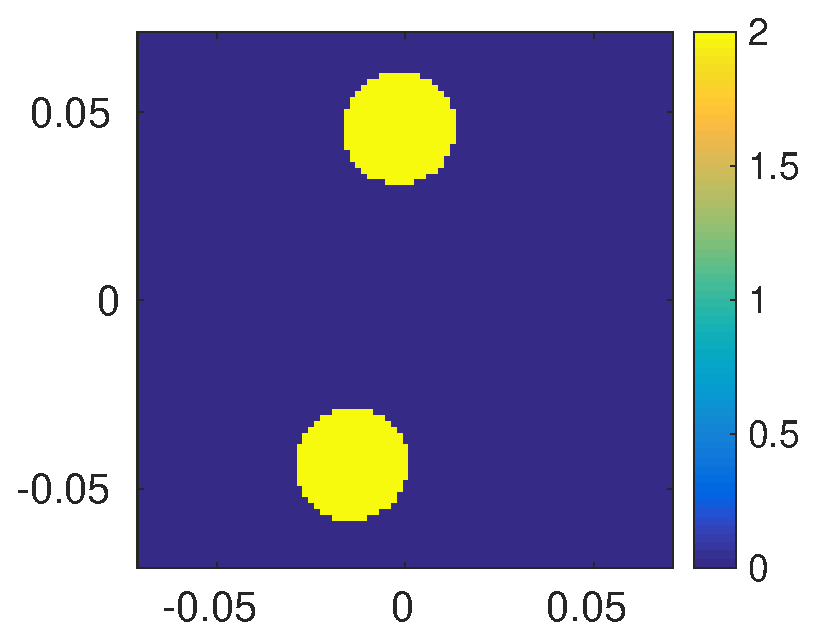
\includegraphics[height=0.22\textwidth]{figs/fig_guideWorkingFresnelContrast}
  }
\end{subcaptionbox}\hspace{2em}
\begin{subcaptionbox}{Real-world data.
   \label{fig:guide:WorkingFresnelMat}}[0.28\textwidth]{
   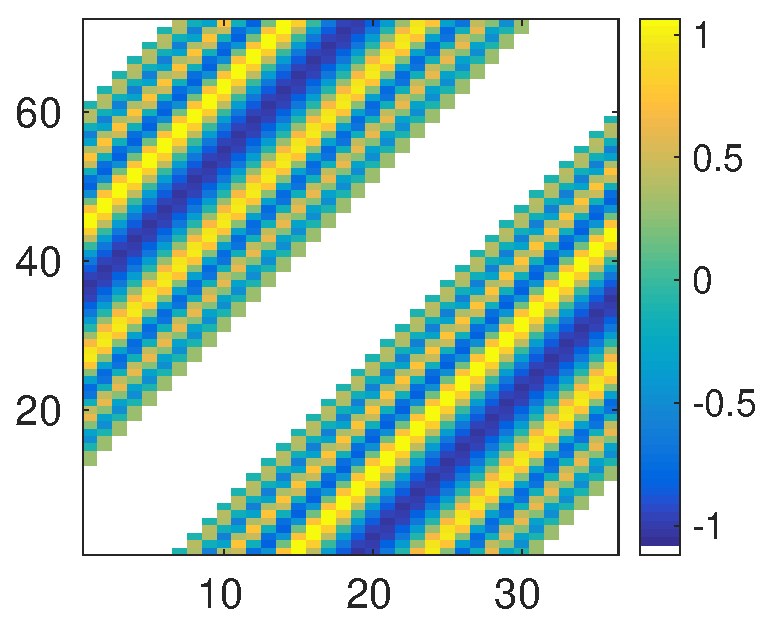
\includegraphics[height=0.22\textwidth]{figs/fig_guideWorkingFresnel}
  }
\end{subcaptionbox}
\caption{Working with data from Institute Fresnel. 
\subref{fig:guide:WorkingFresnelContrast}~Real part of two dielectrics' true contrast from Institute Fresnel data set generated by Lst.~\ref{lst:guideWorkingFresnelContrast}. (The positions were manually corrected.) 
\subref{fig:guide:WorkingFresnelMat}~Result of Lst.~\ref{lst:guideWorkingFresnel}. Some measurements of the incident field are missing due to the experimental set-up (transmitter and receiver have a minimal distance).}
\label{fig:guide:workingFresnel}
\end{figure}

As one of its core features \IPscatt supports users in loading and working with real-world data from Institute Fresnel. The experimental data from Institute Fresnel comprises three opuses, see~(\footnote{\url{http://www.fresnel.fr/3Ddatabase/database.php} (Accessed: 20160921).}). 
The corresponding article to the first opus is~\cite{Belkebir2001} and the supplementary data is available at~(\footnote{\url{http://dx.doi.org/10.1088/0266-5611/17/6/301} (Accessed: 20160921).}). Likewise, the corresponding article to the second opus is~\cite{Geffrin2005} and the supplementary data is available at~(\footnote{\url{http://dx.doi.org/10.1088/0266-5611/21/6/S09} (Accessed: 20160921).}). The user must store the \textsf{*.exp}-files of the first opus in the directory \textsf{inexpdata/fresnel\_opus\_1} and the \textsf{*.exp}-files of the second opus in the directory \textsf{inexpdata/fresnel\_opus\_2} since \IPscatt expects them there.

To read the experimental data the file \textsf{readRAWData.m} is provided in the folder \textsf{proc/expData}. This routine can be used independently of \IPscatt. Note that \IPscatt supports data with transverse magnetic (TM) polarization (instead of transverse electric, TE), because the Helmholtz equation only models electromagnetic waves in the case of TM, see e.g.~\cite{Colton2013}.

\paragraph{Example} Lst.~\ref{lst:guideWorkingFresnelContrast} generates the true contrast of two dielectrics resulting in Fig.~\ref{fig:guide:WorkingFresnelContrast}. The corresponding TM polarized data is loaded by Lst.~\ref{lst:guideWorkingFresnel}. The output is shown in Fig.~\ref{fig:guide:WorkingFresnelMat}.

\begin{lstlisting}[caption={True contrast of two dielectrics (\emph{source code}: \textsf{guides/guideWorkingFresnelContrast.m}).},label=lst:guideWorkingFresnelContrast]
init;
guideSetGrid;
q2D = fresnel_op1_twodielTM(seti.gridROI(1,:), seti.gridROI(2,:),seti);
x = seti.gridROI(1,:); y = seti.gridROI(2,:);
imagesc(x,y,real(reshape(q2D,[seti.nROI seti.nROI]))); axis xy; colorbar;
\end{lstlisting}

\begin{lstlisting}[caption={Reading data from Institute Fresnel (\emph{source code}: \textsf{guides/guideWorkingFresnel.m}).},label=lst:guideWorkingFresnel]
init;
filename = 'inexpdata/fresnel_opus_1/twodielTM_8f.exp';
[uTotRX, uIncRX, frequencies, rTX, nTX, rRX, nRX] = readRAWData(filename);
imagesc(real(uIncRX(:,:,1))); colorbar; axis xy;
\end{lstlisting}

\paragraph{Input and Output Arguments of \textsf{readRAWData}} The input argument \textsf{filename} of the routine \textsf{readRAWData} is the path to the file with real-world data from Institute Fresnel. The outputs are:

\noindent\begin{tabular}[t]{p{1.6cm} p{14cm}}
 \textsf{nTX} & Number of transmitters.\\
 \textsf{nRX} & Number of receivers.\\
 \textsf{rTX} & Radius of the circle on which the transmitters are arranged (in meters).\\
 \textsf{rRX} & Radius of the circle the receivers are arranged on (in meters).\\
 \textsf{frequencies} & Available frequencies as a vector of size \emph{number of frequencies} $\times$ $1$.\\
 \textsf{uIncRX} & Incident field (i.e. without any obstacle) at receivers' positions for each transmitter and each frequency (complex array of size \textsf{nRX} $\times$ \textsf{nTX} $\times$ \emph{number of frequencies}).\\
 \textsf{uTotRX} & Total field (i.e. with an obstacle) at receivers' positions for each transmitter and each frequency (complex array of size \textsf{nRX} $\times$ \textsf{nTX} $\times$ \emph{number of frequencies}).
\end{tabular}

%%

\subsection{Guide: Matching the Incident Fields of Institute Fresnel's Data}\label{sec:guide:matchIncField}

Institute Fresnel provides real-world data of the incident fields at the receivers' positions. For further computations we are actually interested in the corresponding incident field in a region instead of the incident field at the receivers' positions. Assuming point sources at the transmitters' positions this matching is achieved by the function \textsf{matchIncField}, that only works in 2D. For this matching we follow \cite[Sec.~6.2.2]{Gehre2013} and \cite[Sec.~6]{Buergel2017}.

\paragraph{Details of \textsf{matchIncField}} The function \textsf{[uIncROI,errC] = matchIncField(uIncRX,seti,region)} matches incident fields~\textsf{uIncROI} in the computational domain~(CD) or the region of interest~(ROI) (depending on the value of \textsf{region}) corresponding to the data~\textsf{uIncRX}, that contains all incident fields at the receivers' positions. This matching is done by computing the coefficients of the two-dimensional radiating series solutions to the Helmholtz equation, that fits the data at the best in a least-squares sense. Furthermore, it computes the relative error \textsf{errC} of the matched incident field at the receivers' positions for each incident field.

\paragraph{Input Arguments of \textsf{matchIncField}} Remember that \IPscatt expects a two-dimensional problem for matching, i.e. \textsf{seti.dim = 2}. 
Further input arguments are the number of transmitters \textsf{seti.incNb}, the wave number \textsf{seti.k}, the transmitters' positions \textsf{seti.incPnts} (matrix of size 2 $\times$ \textsf{seti.incNb})---e.g. \textsf{seti.incPnts = [5~-2; 0~4]} describes coordinates $(5,0)$ and $(-2,4)$---, the receivers' positions \textsf{seti.measPnts} (matrix of size 2 $\times$ \textsf{seti.measNb}), the grid of the region of interest (ROI) \textsf{seti.gridROI} (if \textsf{region = 'ROI'}) (matrix of size \textsf{seti.dim} $\times$ $\textsf{seti.nROI}^2$) or the grid of the computational domain (CD) \textsf{seti.grid} (if \textsf{region = 'CD'}) (matrix of size \textsf{seti.dim} $\times$ $\textsf{seti.nCD}^2$). The other input arguments are:

\noindent\begin{tabular}[t]{p{2cm} p{13.6cm}}
 \textsf{seti.nuMax} & Approximation order (default: 7). (A good choice is essential for a good matching.)\\
 \textsf{uIncRX} & Incident field at receivers' positions for each transmitter (complex matrix of size \textsf{seti.measNb} $\times$ \textsf{seti.incNb}).\\
 \textsf{region} & \textsf{'ROI'} (region of interest) or \textsf{'CD'} (computational domain), usually interesting is \textsf{'ROI'}.
\end{tabular}

\paragraph{Output Arguments of \textsf{matchIncField}}\hfill\\
\noindent\begin{tabular}[t]{p{2cm} p{13.6cm}}
 \textsf{uIncROI} & Incident field in ROI (or CD) for each transmitter (complex matrix of size $\textsf{seti.nROI}^2$ $\times$ \textsf{seti.incNb}).\\
 \textsf{errC} & Stores the relative error of the matched incident field at the receivers' positions for every transmitter (vector of size 1 $\times$ \textsf{seti.incNb}).
\end{tabular}

\paragraph{Example of \textsf{matchIncField}} Lst.~\ref{lst:guideMatchIncField} reads the same data as Lst.~\ref{lst:guideWorkingFresnel}. For the matching of the incident field it picks the data with a frequency of 5\,GHz. The result is shown in Fig.~\ref{fig:guide:matchIncField}. The data reading, the generation of a grid, the transfer of the experimental set-up into the structure array \textsf{seti} including the computation of the wave number and setting transmitters' as well as receivers' positions was moved into the routine \textsf{matchIncFieldTrans}, that is available in \textsf{guides/\allowbreak auxi/\allowbreak matchIncFieldTrans.m}.

\begin{lstlisting}[caption={Matching the incident field (\emph{source code}: \textsf{guides/guideMatchIncField.m}).},label=lst:guideMatchIncField]
init;
[seti,uTotRX,uIncRX,uScaRX] = matchIncFieldTrans('inexpdata/fresnel_opus_1/twodielTM_8f.exp',5*1E9);
seti.nuMax = 7;
[uIncROI,errC] = matchIncField(uIncRX,seti,'ROI');
imagesc(real(reshape(uIncROI(:,6),[seti.nROI seti.nROI]))); colorbar; axis xy;
\end{lstlisting}

\paragraph{Convenience Function \textsf{loadData}} The routine \textsf{loadData} is a convenience function to load data from Institute Fresnel in three steps: Initially, it reads the data by \textsf{readRAWData} as in Sec.~\ref{sec:guide:workingFresnel}. Then it sets geometry and simulation by \textsf{setGeomSim} as in Sec.~\ref{sec:guide:setGeomSim} (considering required settings for Insitute Fresnel's data, in particular the transmitters' and receivers' positions). Finally, it matches the incident field by \textsf{matchIncField}.

\paragraph{Input Arguments of \textsf{loadData}} The input arguments of \textsf{loadData} are fields of the structure array \textsf{seti}. The most important ones are the path to the data given in the field \textsf{seti.fresnelFile} (default: \textsf{'inexpdata/\allowbreak fresnel\_opus\_1/\allowbreak twodielTM\_8f.exp'}) and the chosen frequency \textsf{seti.fresnelFreq} (default: \textsf{5*1E9}, i.e. 5\,GHz). It is recommended to set all required fields in a consistent manner before executing \textsf{loadData} by setting \textsf{seti.expSetup = 'fresnel'} and using \textsf{checkConsisExpData}. This comprises the parameter \textsf{seti.nuMax}, that was introduced just above, and the input arguments \textsf{seti.rCD} as well as \textsf{seti.nCD}, that are associated to the grid, see Sec.~\ref{sec:guide:setGrid} (as input arguments of \textsf{setGrid}). In particular, some fields are reseted in order to ensure consistency with Institute Fresnel's data, that requires a two-dimensional problem, point sources and near field data. Therefore the routine sets \textsf{seti.dim = 2}, \textsf{seti.incType =  'pointSource'} and \textsf{seti.measType = 'nearField'}.

\paragraph{Output Arguments of \textsf{loadData}} The most important output arguments of \textsf{loadData} are the following.

\noindent\begin{tabular}[t]{p{2.3cm} p{13.3cm}}
\textsf{seti.incNb}   & Number of transmitters.\\
\textsf{seti.measNb}  & Number of receivers.\\
\textsf{seti.radSrc}  & Radius of the circle on which the transmitters are arranged (in meters).\\
\textsf{seti.radMeas} & Radius of the circle on which the receivers are arranged (in meters).\\
\textsf{seti.k}       & Wave number ($k = 2 \pi f/c$ with frequency $f$ and light velocity $c$ in vacuum).\\
\textsf{seti.FmeasDelta} & Data, i.e. the scattered field at the receivers' positions for each transmitter (complex matrix of size $\textsf{seti.measNb} \times \textsf{seti.incNb}$).\\
\textsf{seti.incField} & Incident field in ROI for each transmitter
  (complex matrix of size $\textsf{seti.nROI}^2 \times \textsf{seti.incNb}$). 
  (This field is \textsf{uIncROI} divided by the infinitesimal element \textsf{seti.dSInc}, see Output Arguments of \textsf{matchIncField} for \textsf{uIncROI} and Sec.~\ref{sec:guide:expSetup} for \textsf{seti.dSInc}.)
\end{tabular}

\paragraph{Example of \textsf{loadData}} Lst.~\ref{lst:guideLoadData} demonstrates an application of \textsf{loadData}.

\begin{lstlisting}[caption={Process Institute Fresnel's data with \textsf{loadData} (\emph{source code}: \textsf{guides/guideLoadData.m}).},label=lst:guideLoadData]
init;
seti.expData = 'fresnel';
seti.rCD = 0.2; seti.nCD = 256;
seti.fresnelFreq = 5*1E9; seti.fresnelFile = 'inexpdata/fresnel_opus_1/twodielTM_8f.exp';
seti.nuMax = 7;
seti = checkConsisExpData(seti,1);
seti = loadData(seti);
imagesc(real(seti.G(seti.incField(:,6)))); colorbar; axis xy;
\end{lstlisting}

\begin{figure}
\centering
\begin{subcaptionbox}{\textsf{uIncROI}.
  \label{fig:guide:matchIncField}}[0.31\textwidth]{
  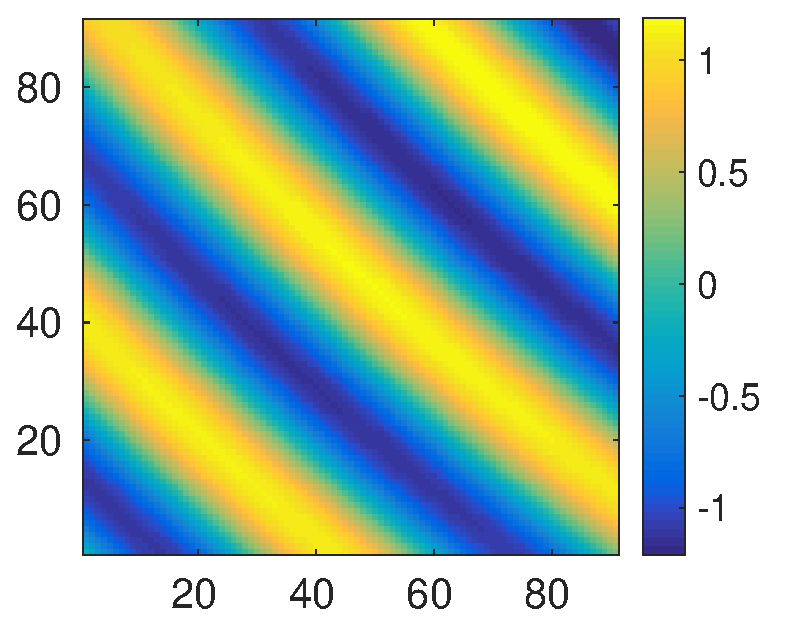
\includegraphics[height=0.22\textwidth]{figs/fig_guideMatchIncField}
  }
\end{subcaptionbox}
\begin{subcaptionbox}{\textsf{seti.incField}.
  \label{fig:guide:LoadData}}[0.31\textwidth]{
  \includegraphics[height=0.22\textwidth]{figs/fig_guideLoadData}
  }
\end{subcaptionbox}
\caption{Matched incident field of the \nth{6} transmitter in the region of interest as \textsf{uIncROI} in~\subref{fig:guide:matchIncField} and scaled as \textsf{seti.incField} in~\subref{fig:guide:LoadData} as generated by Lst.~\ref{lst:guideMatchIncField} and~\ref{lst:guideLoadData}.}
\label{fig:guide:FresnelMatch}
\end{figure}

\paragraph{Example of \textsf{setData} in the Case of Institute Fresnel's Data} We have already seen that the convenience function \textsf{setData} comprises to set geometry as well as simulation and to add noise to the data, see Lst.~\ref{lst:guideSetData} in Sec.~\ref{sec:guide:addNoise}. Apart from this generation of synthetic data the routine \textsf{setData} is useful to deal with real-world data from Institute Fresnel because it employs \textsf{checkConsisExpData} and \textsf{loadData} in the case of \textsf{seti.expData = 'fresnel'}. Therefore Lst.~\ref{lst:guideSetDataFresnel} is the same as Lst.~\ref{lst:guideLoadData} except for the geometry.

\begin{lstlisting}[caption={Process Institute Fresnel's data with \textsf{setData} (\emph{source code}: \textsf{guides/guideSetDataFresnel.m}).},label=lst:guideSetDataFresnel]
init;
seti.expData = 'fresnel';
seti.fresnelFreq = 5*1E9; seti.fresnelFile = 'inexpdata/fresnel_opus_1/twodielTM_8f.exp';
seti = setData(seti);
\end{lstlisting}

%%

\subsection{Guide: Variational Reconstruction}\label{sec:guide:recon}

Before executing the variational reconstruction by the routine \textsf{recon} we have to set the fields of the structure array \textsf{seti} for the forward operator in a consistent manner. Therefore it is recommended to use the function \textsf{setData}, see Sec.~\ref{sec:guide:addNoise} and~\ref{sec:guide:matchIncField}. Furthermore, the routine \textsf{recon} requires reconstruction-specific fields of \textsf{seti}. For this preparation \IPscatt provides the function \textsf{setRecon}, which is the subject of the first part of this guide.

\paragraph{Details of \textsf{setRecon}} The routine \textsf{setRecon} consists of the functions \textsf{setInvType}, \textsf{checkConsisRec} and \textsf{setFuncsPda} with the mentioned structure array \textsf{seti} as input and output argument.

In \textsf{setInvType} some default parameters for the variational reconstruction are set in dependent on the inversion method number \textsf{seti.invNo}. We will confine ourselves to discussing the default choice of \textsf{seti.invNo = 6}. In this case \IPscatt uses the variational reconstruction scheme which is described in the \emph{algorithm paper} and in detail in \cite[Sec.~4]{Buergel2017}. As the reconstruction scheme relies on the primal-dual algorithm, see~\cite{Chambolle2011}, the reconstruction's type is chosen as \textsf{seti.inv = 'pda'}. Further, the minimization functional for the inner iteration is essentially~\eqref{eq:minFuncSimple} and the assignment $F(Kh) = f_\dis(h) + f_\sparse(h)$ as well as $G(h) = f_\sparse(h) + f_\phy(h)$ is used for the required split of the minimization functional into two parts $F$ and $G$ with $\min_{h \in \ROID} F(Kh) + G(h)$, where $K$ is a continuous linear operator.

The routine \textsf{setFuncsPda} defines the functions for the primal-dual algorithm, i.e. essentially $f_\dis$, $f_\sparse$, $f_\gra$, $f_\phy$ as well as $K_\dis$ and $K_\gra$ (the parts of the linear operator $K$) as fields \textsf{fd}, \textsf{fs}, \textsf{fg}, \textsf{fp}, \textsf{Kd}, \textsf{Kg} of the structure array \textsf{seti} and their adjoints \textsf{KdAdj} and \textsf{KgAdj}, see~\textsf{setFuncsPda.m}.

\paragraph{Output and Optional Input Arguments of \textsf{setRecon}} If they are not already defined, the function \textsf{setRecon} sets all reconstruction-specific fields of \textsf{seti}. This is done in a consistent and appropriate manner. In particular, the following main fields are set.

\noindent\begin{tabular}[t]{p{2.3cm} p{13.3cm}}
\textsf{seti.alpha} & Regularization parameter $\alpha$ for the sparsity penalty (default: 500), see~\eqref{eq:minFuncSimple}.\\
\textsf{seti.beta} & Regularization parameter $\beta$ for the total variation penalty (default: $10^{-5}$), see~\eqref{eq:minFuncSimple}.\\
\textsf{seti.tau} & Tolerance parameter $\tau$ of the discrepancy principle (default: $2.5$), see~\eqref{eq:morozov}.\\
\textsf{seti.physBounds} & Bounds for real/imaginary part of contrast: $[a, b, c, d]$ (default: [-1,3,0,3]), see~\eqref{eq:minFuncSimple}.\\
\textsf{seti.useDis} & 0 or 1 (default): Set this to 1 to stop the outer iterations by the discrepancy principle.\\
\textsf{seti.nOut} & Maximal number of the outer iterations (default: 30).\\
\textsf{seti.pdaN} & Number of the inner iterations (primal-dual algorithm) (default: 50).\\
\textsf{seti.useTolOut} & 0 (default) or 1: Set this to 1 to stop the inner iterations by the outer tolerance principle, see stopping strategy~1 in Sec.~\ref{sec:guide:stopping}.\\
\textsf{seti.useTolIn} & 0 (default) or 1: Set this to 1 to stop the inner iterations (primal-dual algorithm) by the inner tolerance principle, see stopping strategy~2 in Sec.~\ref{sec:guide:stopping}.
\end{tabular}

For more information see~\textsf{setRecon.m}, \textsf{setInvType.m}, \textsf{checkConsisRec.m} and~\textsf{setFuncsPda.m}.

\paragraph{Details of \textsf{recon}} The routine \textsf{recon} executes the above-mentioned variational reconstruction scheme of the contrast. It uses the functions \textsf{minPda} for the outer and \textsf{pda} for the inner iteration. The relative discrepancy of the reconstructed contrast $q^{(m)}$ after $m$ outer iterations is $\mathrm{dis}(m):= \|\F(q^{(m)})-\msdata^\delta\|_\fro / \|\msdata^\delta\|_\fro$, where $m = 1, 2, \ldots$ is the index of the outer iteration. Furthermore, the relative error is $\mathrm{err}(m) := \|q^{(m)}-q_\mathrm{exa}\|_2 / \|q_\mathrm{exa}\|_2$, where $q_\mathrm{exa}$ is the exact contrast.

Additionally, \textsf{recon} provides a way to load the reconstruction result from a previous computation---to plot and save reconstruction-depending figures---and offers the opportunity to save discrepancies, errors and reconstruction results. This is helpful for prototyping purposes and is presented in Sec.~\ref{sec:guide:convenience}.

\paragraph{Input Argument of \textsf{recon}} As already mentioned the routine \textsf{recon} requires fields of the structure array \textsf{seti}, that were defined in \textsf{setData}, see Sec.~\ref{sec:guide:addNoise} and~\ref{sec:guide:matchIncField}, and \textsf{setRecon}.

\paragraph{Output Argument of \textsf{recon}} The most important fields of the output argument \textsf{seti} are the following.

\noindent\begin{tabular}[t]{p{2.3cm} p{13.3cm}}
\textsf{seti.qROIcomp} & Computationally reconstructed contrast (complex vector of size $\textsf{seti.nROI}^d \times 1$ with $d = \textsf{seti.dim}$).\\
\textsf{seti.iOutStop} & Stop index of outer iterations.\\
\textsf{seti.dis} & Relative discrepancy for each outer iteration (vector of size $1 \times \textsf{seti.nOut}$).\\
\textsf{seti.err} & Relative error for each outer iteration (vector of size $1 \times \textsf{seti.nOut}$).
\end{tabular}

\begin{figure}
\centering
\begin{subcaptionbox}{\textsf{seti.qROIexact}.
   \label{fig:guide:recon1}}[0.28\textwidth]{
   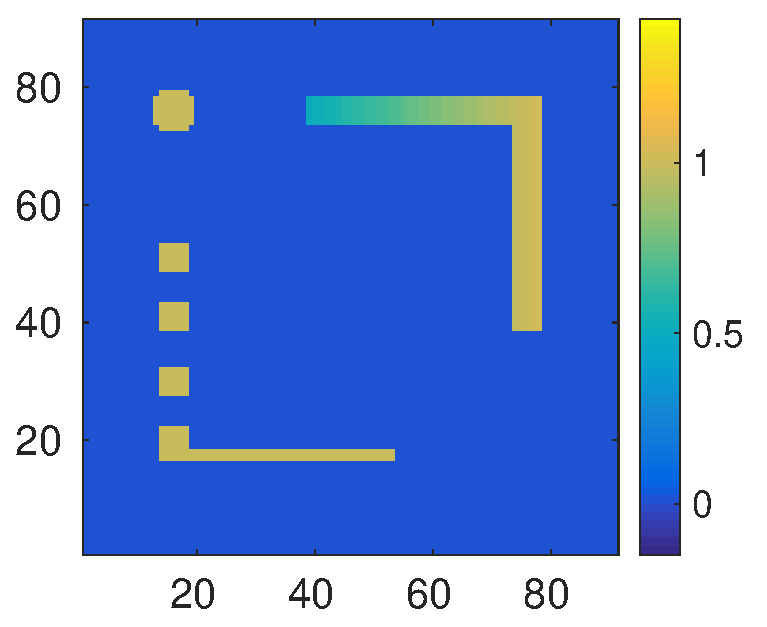
\includegraphics[height=0.22\textwidth]{figs/fig_guideRecon1}
  }
\end{subcaptionbox}
\begin{subcaptionbox}{\textsf{seti.qROIcomp}.
   \label{fig:guide:recon2}}[0.28\textwidth]{
   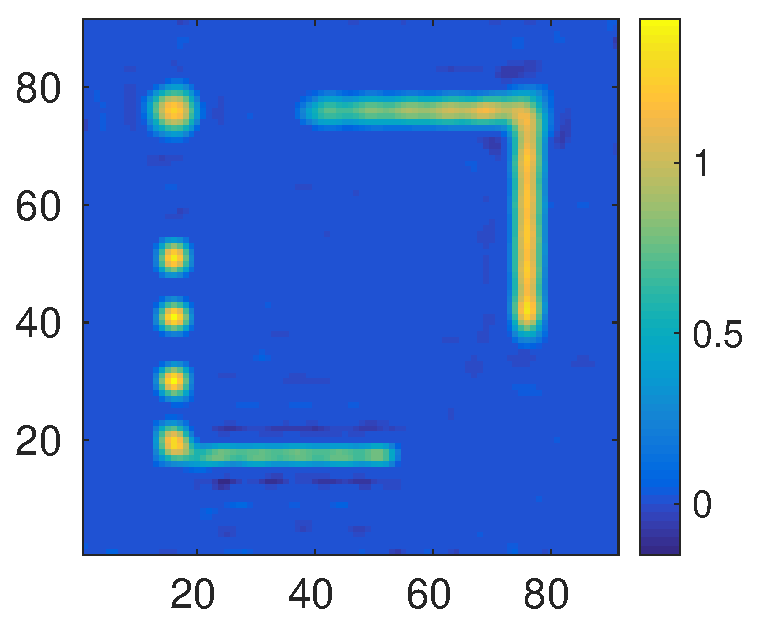
\includegraphics[height=0.22\textwidth]{figs/fig_guideRecon2}
  }
\end{subcaptionbox}
\caption{Real part of the exact and reconstructed contrast in~\subref{fig:guide:recon1} and~\subref{fig:guide:recon2} as generated by Lst.~\ref{lst:guideRecon}.}
\label{fig:guide:recon}
\end{figure}

\paragraph{Example} Lst.~\ref{lst:guideRecon} reconstructs the contrast from perturbed data and compares it with the exact one (\textsf{seti.qROIexact}, see Sec.~\ref{sec:guide:contrast}). The run time is approximately 1\,min and the results are shown in Fig.~\ref{fig:guide:recon}. The reconstruction stops after \textsf{seti.iOutStop} = 11 outer iterations with a relative discrepancy of \textsf{seti.dis(seti.iOutStop)} = 0.024 and a relative error of \textsf{seti.err(seti.iOutStop)} = 0.359. Remember that the number of inner iterations is fixed to 50 by the parameter \textsf{seti.pdaN} in this example; see Sec.~\ref{sec:guide:stopping} for more sophisticated methods.

\begin{lstlisting}[caption={Variational reconstruction (\emph{source code}: \textsf{guides/guideRecon.m}).},label=lst:guideRecon]
init;
seti = struct;
seti = setData(seti);
seti = setRecon(seti);
seti = recon(seti);
figure(1); imagesc(real(seti.G(seti.qROIexact))); axis xy; colorbar;
figure(2); imagesc(real(seti.G(seti.qROIcomp))); axis xy; colorbar;
\end{lstlisting}

Lst.~\ref{lst:guideReconDetails} computes the same as Lst.~\ref{lst:guideRecon}, but displays messages of the functions, because of the choice of the additional input argument \textsf{dispDepth} to~4. This additional input argument was already mentioned in~Sec.~\ref{sec:guide:setGeomSim}. For the details we refer to Sec.~\ref{sec:guide:convenience}.

\begin{lstlisting}[caption={Variational reconstruction with display of messages (\emph{source code}: \textsf{guides/guideReconDetails.m}).},label=lst:guideReconDetails]
init; seti = struct; seti = setData(seti,4); seti = setRecon(seti,4); seti = recon(seti,4);
\end{lstlisting}

\begin{figure}
\centering
\begin{subcaptionbox}{\textsf{seti.qROIexact}.
   \label{fig:guide:recon3D1}}[0.28\textwidth]{
   \includegraphics[height=0.26\textwidth]{figs/fig_guideRecon3D1}
  }
\end{subcaptionbox}
\begin{subcaptionbox}{\textsf{seti.qROIcomp}.
   \label{fig:guide:recon3D2}}[0.28\textwidth]{
   \includegraphics[height=0.26\textwidth]{figs/fig_guideRecon3D2}
  }
\end{subcaptionbox}
\caption{Real part of the exact and reconstructed contrast in~\subref{fig:guide:recon3D1} and~\subref{fig:guide:recon3D2} as generated by Lst.~\ref{lst:guideRecon3D}. The reconstruction stops after 9 outer iterations with a relative discrepancy of 0.012 and a relative error of 0.659. The run time was~4.1\,h.}
\label{fig:guide:recon3D}
\end{figure}

\paragraph{Example in Three Dimensions} Lst.~\ref{lst:guideRecon3D} shows a three-dimensional reconstruction of two tripods. The results are plotted in Fig.~\ref{fig:guide:recon3D}. Note that the used convenience function \textsf{contourPlotROI} was already mentioned in Sec.~\ref{sec:guide:contrast}. Furthermore, note that there is no text information displayed during the run time of several hours; see Lst.~\ref{lst:guideReconDetails} to change this behavior.

\begin{lstlisting}[caption={Variational reconstruction in three dimensions (\emph{source code}: \textsf{guides/guideRecon3D.m}).},label=lst:guideRecon3D]
init;
seti.dim = 3; seti.rCD = 2.0; seti.k = 10;
seti.contrast = 'twoTripods3D';
seti.incNb = 35; seti.measNb = 35;
seti.radSrc = 5; seti.radMeas = 5;
seti.tau = 1.25;
seti = setData(seti); seti = setRecon(seti); seti = recon(seti);
figure(1); contourPlotROI(seti.qROIexact, seti, 'real');
figure(2); contourPlotROI(seti.qROIcomp, seti, 'real');
\end{lstlisting}

For more information about the variational reconstruction see~\textsf{recon.m}.

%%

\subsection{Guide: Stopping Strategies of the Inner Iteration}\label{sec:guide:stopping}

In Sec.~\ref{sec:guide:recon} the reconstruction uses a fixed number of inner iterations as defined by \textsf{seti.pdaN}. To use more sophisticated stopping criteria, mentioned in the \emph{algorithm paper} and explained in~\textsf{minTolOut.m} and~\textsf{minTolIn.m}, \IPscatt provides stopping strategies~1 and~2. They are activated by \textsf{seti.useTolOut = 1} and \textsf{seti.useTolIn = 1}.
If a stopping strategy is activated and strategy-dependent fields of \textsf{seti} are not defined, they are set to default values in \textsf{setRecon} (to be precisely in \textsf{checkConsisRec}). 
A field, that is set in both cases, is the maximal number of inner iterations by \textsf{seti.pdaNmax} (default: $250$).

In the first case (stopping strategy 1) the outer tolerance (default: $0.05$) in \textsf{seti.relDisTol} is set too, see~\textsf{minTolOut.m}.
%
In the second case (stopping strategy 2), these additional fields of \textsf{seti} are \textsf{ThetaStart} (default: $0.925$), \textsf{ThetaMax} (default: $0.95$) and \textsf{TolGamma} (default: $0.90$) to compute the inner tolerance \textsf{ThetaiOut}, see~\textsf{minTolIn.m}. (The second strategy follows an inexact stopping rule for a Newton-like method, see~\cite{Rieder2001}.)

\paragraph{Example} Lst.~\ref{lst:guideStop} reconstructs as in Lst.~\ref{lst:guideRecon}, but with activated stopping strategy~1. 
To use the second stopping strategy in this example replace \textsf{seti.useTolOut = 1} by \textsf{seti.useTolIn = 1}.

\begin{lstlisting}[caption={Variational reconstruction with stopping strategy 1 (\emph{source code}: \textsf{guides/guideStop.m}).},label=lst:guideStop]
init;
seti.useTolOut = 1;
seti = setData(seti); seti = setRecon(seti); seti = recon(seti);
\end{lstlisting}

%%

\subsection{Guide: Setting Up Test Bench for Variational Reconstruction}\label{sec:guide:convenience}

The proceeding to identify the contrast was described in Lst.~\ref{lst:guideReconDetails} in Sec.~\ref{sec:guide:recon}. It is a common scenario for the inverse medium problem. To omit a repetition of these steps \IPscatt provides the convenience function \textsf{start}. In addition to the steps in Lst.~\ref{lst:guideReconDetails}, this function plots the results and saves these figures as well as other files in a subfolder of the directory \textsf{output}. Note that \textsf{start} closes all figures and usually clears almost all variables.

\paragraph{Details of \textsf{setInput}} The just-mentioned typical closing of figures and clearing of variables are tasks of \textsf{setInput}. Additionally, it creates a directory with path \textsf{seti.dirname} in the folder \textsf{output} for the later storage of figures and other files. Note that \textsf{setInput} evaluates the input argument \textsf{inseti} (in the case of existence) to load input parameters, i.e. fields of the structure array \textsf{seti}, that were saved in the corresponding file.

\paragraph{Input Arguments of \textsf{setInput}} Note that all input arguments are optional.

\noindent\begin{tabular}[t]{p{2.4cm} p{13.2cm}}
\textsf{inseti} & File's name in the folder \textsf{inseti} containing input parameters as fields of the structure array \textsf{seti}.
\end{tabular}

For the input arguments \textsf{usevaralpha}, \textsf{usevarbeta} and \textsf{usevardelta} (each 0 or 1) we refer to Sec.~\ref{sec:guide:various}. 
%
The following fields of the structure array \textsf{seti} can be set in the file whose name the variable \textsf{inseti} refers to. They are set to default values if they are not defined by the user. We omit to explain \textsf{seti.dirSuffix}, \textsf{seti.dirSuffixAdd} and \textsf{seti.fileSuffix} because it is clear from the context.

\noindent\begin{tabular}[t]{p{2.4cm} p{13.2cm}}
\textsf{seti.dirOutput} & Name of folder in which directories for output files/figures are created (default: \textsf{'output'}).\\
\textsf{seti.dirDatetime} & Date and time separated by the character ``T'' in the format \textsf{<yyyyMMdd>T<HHmmss>}, e.g. 20161006T105735.\\
\textsf{seti.dirname} & Dirname for files and figures from current computation, default:\newline
  \textsf{<seti.dirOutput>/<seti.datetime>\_<seti.inseti><seti.dirSuffix><seti.dirSuffixAdd>}\newline
  If \textsf{seti.inseti} is empty, \textsf{'noinseti'} is inserted; e.g. 
  \textsf{output/\allowbreak 20161006T102740\_noinseti}.\\
\end{tabular}

\paragraph{Output Arguments of \textsf{setInput}} Most fields of \textsf{seti} were already described as input arguments. Note that \textsf{seti.inseti = inseti} or is empty, if \textsf{inseti} does not exist.

\paragraph{Example} Before we discuss the example we recommend to start \MATLAB with the option \textsf{nodisplay} as indicated in Lst.~\ref{lst:nodisplay} because this avoids verbose program output. Regardless, the related figures are stored.

\begin{lstlisting}[caption={Using \MATLAB with the option \textsf{nodisplay}.},label=lst:nodisplay]
matlab -nodisplay
\end{lstlisting}

To get an idea of \textsf{start} its essential functions are demonstrated in Lst.~\ref{lst:guideReconOut}.

\begin{lstlisting}[caption={Variational reconstruction with messages and storing of figures/files (\emph{source code}: \textsf{guides/guideReconOut.m}).},label=lst:guideReconOut]
inseti = 'exampleMod'; init; setInput;
seti = setData(seti,4,2); seti = setRecon(seti,4,2); seti = recon(seti,4,2);
\end{lstlisting}

As already mentioned all input parameters are stored in the structure array \textsf{seti}. In this example they were loaded from the file \textsf{inseti/exampleMod.m}. Changes of parameters must be done in such a file, since almost all variables are cleared in the routine \textsf{setInput}. Therefore \IPscatt provides the file \textsf{example.m}, that contains the most important parameters and a short explanation. The user can change this file or create own files and name them. However, it is important to choose names other than existing functions in \IPscatt. 

Messages in Lst.~\ref{lst:guideReconOut} are displayed because \textsf{dispDepth} was set to~4. This already-mentioned additional input argument controls the depth of displayed messages by an integer between 0 and~5 (messages are suppressed by~0). Furthermore, the optional input argument \textsf{out} was set to~2 to plot and save figures as well as files; any storing would be suppressed by~1, plotting would be suppressed by~0. The plots are stored in the created subfolder in the directory \textsf{output}. 
The most important figures are explained in Fig.~\ref{fig:guide:convenience}. A full list of stored figures is in~\textsf{start.m}. 
A folder with the current date and time is created for each computation and figures are saved as \textsf{png} by default (other formats are possible, see~\textsf{example.m}).

To get the same result as in Lst.~\ref{lst:guideReconOut} it is easier to use the convenience function \textsf{start} as in Lst.~\ref{lst:guideStart}.

\begin{lstlisting}[caption={Convenience function \textsf{start}.},label=lst:guideStart]
inseti = 'exampleMod'; start;
\end{lstlisting}

It is also possible just to use \textsf{start} without defining \textsf{inseti}. Then default input parameters are used. 
%
Of course, it is possible to use \textsf{setInput} and avoid \textsf{inseti} by defining fields of \textsf{seti} after \textsf{setInput} as demonstrated in Lst.~\ref{lst:guideSeti}.

\begin{lstlisting}[caption={Control the running of all processes (\emph{source code}: \textsf{guides/guideSeti.m}).},label=lst:guideSeti]
init; setInput;
seti.contrast = 'cornerBallSparseMod2D';
seti = setData(seti,4,2); seti = setRecon(seti,4,2); seti = recon(seti,4,2);
\end{lstlisting}

\begin{figure}
\centering
\begin{subcaptionbox}{Transmitters and receivers.
  \label{fig:convenience:transRecei}}[0.31\textwidth]{
  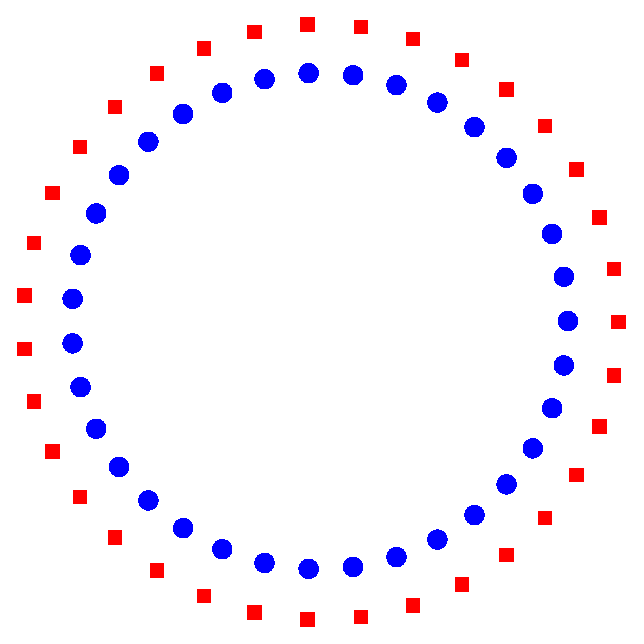
\includegraphics[height=0.22\textwidth]{figs/fig_exampleMod_01_iOut_00}
  }
\end{subcaptionbox}
\begin{subcaptionbox}{Predefined contrast.
  \label{fig:convenience:predefined}}[0.31\textwidth]{
  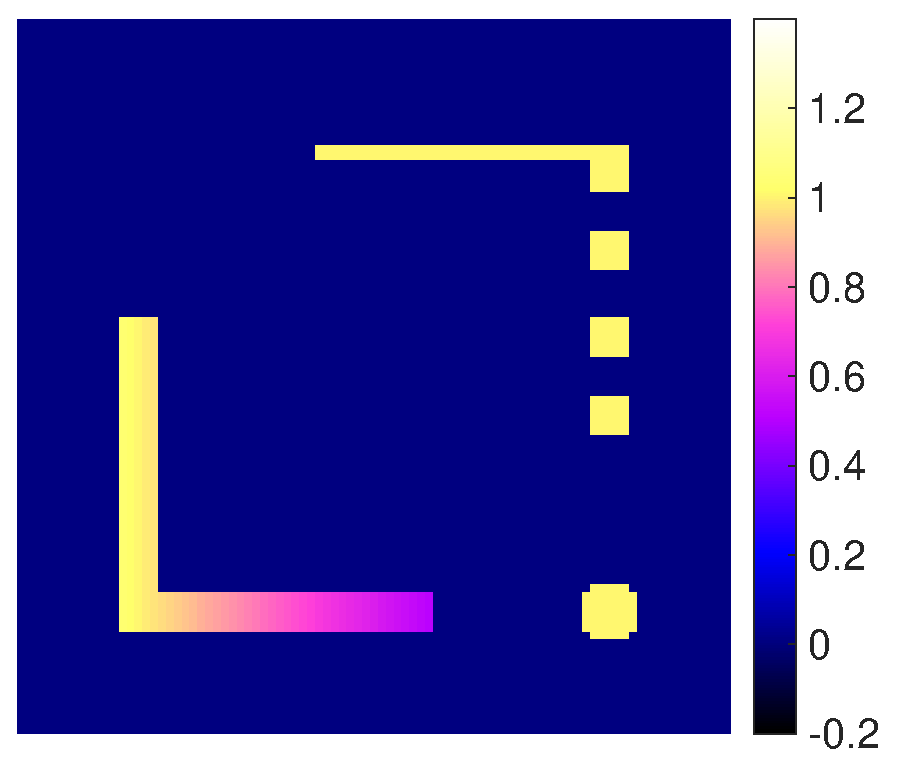
\includegraphics[height=0.22\textwidth]{figs/fig_exampleMod_02_iOut_00}
  }
\end{subcaptionbox}
\begin{subcaptionbox}{Reconstructed contrast.
  \label{fig:convenience:recon}}[0.31\textwidth]{
  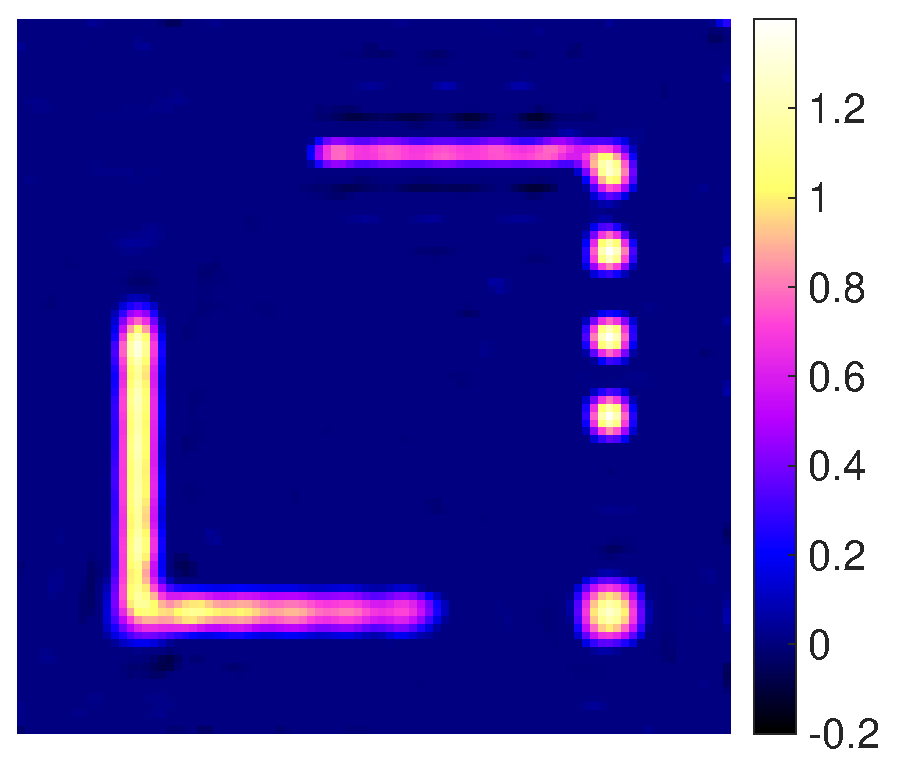
\includegraphics[height=0.22\textwidth]{figs/fig_exampleMod_14_iOut_11}
  }
\end{subcaptionbox}
\caption{The most important figures generated by \textsf{start} of \IPscatt, see Lst.~\ref{lst:guideStart}. 
\subref{fig:convenience:transRecei}~The positions of the transmitters (blue circles) and receivers (red squares) (filename: \textsf{fig\_01\_iOut\_00.png}). 
\subref{fig:convenience:predefined}~The real part of the predefined contrast (filename: \textsf{fig\_02\_iOut\_00.png}). 
\subref{fig:convenience:recon}~The real part of the reconstruction (filename: \textsf{fig\_14\_iOut\_11.png}). (Note that the number \textsf{11} changes because it is the number of the outer iterations.) The relative noise level was $\delta = 0.01$. The run time was 4\,min, the relative discrepancy 0.028 and the relative error 0.358.}
\label{fig:guide:convenience}
\end{figure}

\paragraph{Store and Load Simulated Data} The routine \textsf{setData} provides a way to save and load the exact and perturbed data \textsf{seti.FmeasExact} as well as \textsf{seti.FmeasDelta} for further computations. This is, for example, helpful to avoid the ``inverse crime'', explained in Sec.~\ref{sec:guide:invCrime}. 
%
They are saved as \textsf{FmeasExact} and \textsf{FmeasDelta} in the file \textsf{save\_Fmeas.mat} inside the folder of the path \textsf{seti.dirname} if no field \textsf{expData} in \textsf{seti} exists and \textsf{out} equals~2.

To load them, the path in \textsf{seti.loadFmeas} has to bet set. (If the field is empty, i.e. in the code \textsf{''}, nothing is loaded.) The stored perturbed data is usually used because \textsf{seti.useFmeasDelta} is set to~1 by default. Perturbed data is generated again from the stored exact data if it is set to~0.

\paragraph{Store and Load the Reconstruction} It is also possible to store and load the result of the reconstruction process, e.g. to continue it. The following input arguments belong to \textsf{recon} and \textsf{setRecon} (to be exactly they are in \textsf{checkConsisRec}). However, we mention them here. If the user does not define them, they are set to default values. In addition, the setting is only useful in the case of an existing folder to store the files.

\noindent\begin{tabular}[t]{p{2.8cm} p{12.8cm}}
\textsf{seti.loadqROIcomp} & Path to load a \textsf{mat}-file containing the reconstructed contrast \textsf{qROIcomp} and the number of outer iterations \textsf{iOutStop} (default: empty, i.e. in the code \textsf{''} or \textsf{[]}, then no data is loaded).\\
\textsf{seti.saveqROIcomp} & Path to store the reconstructed contrast. The default filename is essentially \textsf{save\_qROIcomp\_iOutStop.mat} in the same subfolder of \textsf{output} containing the figures.\\
\textsf{seti.savedata} & 0 (default) or 1: If this is set to 1, relative discrepancies, errors, and differences of the iterated contrasts are saved (as \textsf{save\_dis.mat}, \textsf{save\_err.mat} and \textsf{save\_dif.mat}).
\end{tabular}

\paragraph{Example of Storing and Loading the Reconstruction} Lst.~\ref{lst:guideConvReconStoreLoad} does the default reconstruction of perturbed simulated data and creates a new subfolder in the folder \textsf{output}, e.g. \textsf{20170308T143238\_noinseti}. The reconstruction was stopped after 11 outer iterations (by the discrepancy principle) and took 3.5\,min.

\begin{lstlisting}[caption={A reconstruction process to be continued.},label=lst:guideConvReconStoreLoad]
inseti = ''; start;
\end{lstlisting}

Two steps are necessary to continue the reconstruction: First, the computed contrast is loaded by setting \textsf{seti.loadqROIcomp} to \textsf{output/\allowbreak 20170308T143238\_noinseti/\allowbreak save\_qROIcomp\_iOutStop.mat} under the use of \textsf{seti.dirname}, see Lst.~\ref{lst:guideConvReconStoreLoadCont}. Second, the tolerance parameter $\tau = \textsf{seti.tau}$ of the discrepancy principle~\eqref{eq:morozov} is decreased from 2.5 to 2.0; it was set to 2.5 by default in Lst.~\ref{lst:guideConvReconStoreLoad}. Note that some files in this folder are overwritten by new ones. The continued reconstruction is stopped after 21 outer iterations (by the discrepancy principle), i.e. the continuation did outer iterations number 12 to 21.

\begin{lstlisting}[caption={The continuation of Lst.~\ref{lst:guideConvReconStoreLoad} (\emph{source code}: \textsf{guides/guideConvReconStoreLoadCont.m}).},label=lst:guideConvReconStoreLoadCont]
seti.tau = 2.0;
seti.loadqROIcomp = sprintf('%s/save_qROIcomp_iOutStop.mat',seti.dirname);
seti = setRecon(seti,4,2); seti = recon(seti,4,2);
\end{lstlisting}

%%

\subsection{Guide: Avoiding the Inverse Crime}\label{sec:guide:invCrime}

The forward operator is just a physical model of the reality. Therefore the usage of the same forward operator for the generation and inversion of synthetic data leads to reconstructions that are ``too good to be true``, see~\cite{Kaipio2005} or~\cite{Mueller2012}. This problem is known in literature as ``inverse crime'', see~\cite{Colton2013}. 
%
To avoid it we follow \cite[Ch.~2.3.6]{Mueller2012} and generate synthetic data on a fine grid but reconstruct on a coarse grid not sharing common factors, e.g. the computational domain is discretized by $N = 1127$ points in each dimension in 2D ($N = 563$ in 3D) for computing synthetic data and by $N = 256$ for reconstructions (in 2D and 3D), see~\cite[Sec.~5]{Buergel2017}.

Therefore we will consider an example of storing and loading simulated data to avoid the ``inverse crime'': Lst.~\ref{lst:guideConvSimSaveIn}--\ref{lst:guideConvSimLoad} show how to avoid it by generating perturbed data on a fine grid (with 1127 discretization points in each dimension) before preparing the reconstruction on a coarse grid (with 256 points in each dimension). First, to store the data in a folder that does not depend on time, we create a file in the folder \textsf{inseti} to redefine \textsf{seti.dirname}, see Lst.~\ref{lst:guideConvSimSaveIn}.

\begin{lstlisting}[caption={File \textsf{inseti/guideConvSimSaveIn.m} with input parameters to save data.},label=lst:guideConvSimSaveIn]
seti.dirOutput = 'output';
seti.dirname = sprintf('%s/storeLoadSim',seti.dirOutput);
seti.nCD = 1127;
\end{lstlisting}

Second, the source code in Lst.~\ref{lst:guideConvSimSave} involves this file in \textsf{inseti}, such that \textsf{setInput} creates the directory \textsf{storeLoadSim} in the folder \textsf{output} and the routine \textsf{setData} stores the exact and perturbed data in \textsf{output/\allowbreak storeLoadSim/\allowbreak save\_Fmeas.mat}. (This process takes 1\,min.)

\begin{lstlisting}[caption={Simulate data and save them (\emph{source code}: \textsf{inseti/guideConvSimSave.m}).},label=lst:guideConvSimSave]
inseti = 'guideConvSimSaveIn';
init; setInput; seti = setData(seti,4,2);
\end{lstlisting}

It is also possible to use the code snippet \textsf{inseti = 'guideConvSimSaveIn'; start;} to run the whole process including reconstruction and terminate it before the reconstruction starts, i.e. when the message ``\textsf{\#\#~setRecon -- variational reconstruction}'' appears.

Third, \textsf{seti.loadFmeas} is set to the just stored file to load the data as in Lst.~\ref{lst:guideConvSimLoad}. 
%
Afterwards the reconstruction can be started by \textsf{seti = setRecon(seti); seti = recon(seti);}. Note that \textsf{seti.nCD} is set to the default value 256, because the field does not exist. 

\begin{lstlisting}[caption={Load exact and perturbed data (\emph{source code}: \textsf{guides/guideConvSimLoad.m}).},label=lst:guideConvSimLoad]
clear all; init;
seti.loadFmeas = 'output/storeLoadSim/save_Fmeas.mat';
seti = setData(seti);
\end{lstlisting}

The most convenient method to avoid the ``inverse crime'' is: first, create a file in the folder \textsf{inseti} with all desired fields of \textsf{seti}, increase the discretization \textsf{seti.nCD}, e.g. to 1127, and leave \textsf{seti.loadFmeas} empty; second, start the whole process by \textsf{start} and terminate it before the reconstruction starts; third, set in the created file (from the first step) both \textsf{seti.loadFmeas} to the just now stored \textsf{save\_Fmeas.mat} and the discretization \textsf{seti.nCD} to a smaller value, e.g. 256; and fourth, start the whole process by \textsf{start}.

%%

\subsection{Guide: Choosing the Regularization Parameters}\label{sec:guide:various}

A careful selection of the regularization parameters $\alpha$ and~$\beta$ is necessary for a pleasing reconstruction. This requires extensive numerical experiments. Therefore \IPscatt provides the functions \textsf{varalpha} and \textsf{varbeta}. They employ the routine \textsf{start} several times trying to identify the contrast with chosen various inputs of $\alpha$ and~$\beta$.

For example, to try reconstructions with regularization parameter $\alpha$ set to 100, 500 and 1000, it has to be set \textsf{alpha = [100; 500; 1000];} in the file \textsf{varalpha.m}. Afterwards it is started as in Lst.~\ref{lst:guideVarious}. Of course, a file in the folder \textsf{inseti} can be chosen to set deviating values from default.

\begin{lstlisting}[caption={Various regularization parameters.},label=lst:guideVarious]
inseti = ''; varalpha;
\end{lstlisting}

For a systematic search of reasonable regularization parameters we recommend first to set $\alpha = \textsf{seti.alpha} = 0$ and find a suitable $\beta = \textsf{seti.beta}$ and second to look for a proper $\alpha$, see \cite[Sec.~5]{Buergel2017}. 

In addition, \IPscatt provides the routine \textsf{vardelta} to try out different noise levels~$\delta$.

%%

\section{Applications}\label{sec:applications}
We demonstrate the modular design of \IPscatt on three examples: first, the computation of the Born approximation and the scattered field, second, the Born approximation of the inverse medium problem and third, the linearization at a specific contrast. We hope this encourages users of \IPscatt to take parts of it and use them for their own applications.

%

\paragraph{Comparison of Born Approximation and Scattered Field}
%
The Born approximation $u_\born(q) = V(q \cdot u^\Inc)$, see~\cite[Ch.~4.2]{Kirsch2008} or~\cite{Born1926}, is linear and approximates the scattered field $u^\Sca$ for relatively small wave numbers $k = \textsf{seti.k}$, see Fig.~\ref{fig:born}, by ignoring the repeated scattering inside the region of interest. (The source code generating Fig.~\ref{fig:born} can be found in \textsf{guides/\allowbreak guideBornk.m}.) 
In Lst.~\ref{lst:guideBorn} the volume potential operator $V$, see~\eqref{eq:VPs}, is defined and the Born approximation \textsf{uBorn} is computed for a given incident field $u^i = \textsf{uIncROI}$ and contrast $q = \textsf{qROI}$. Further, the scattered field $u^\Sca = \textsf{uScattROI}$ is computed by solving the Lippmann-Schwinger integral equation~\eqref{eq:LSI}. Of course, if the Born approximation was computed, the result can also used as second input argument of \textsf{solveLippmannSchwinger}.

\begin{lstlisting}[caption={Comparison of Born approximation and scattered field (\emph{source code}: \textsf{guides/guideBorn.m}).},label=lst:guideBorn]
% Generate uIncROI (e.g. of 1st transmitter) and qROI:
init; seti.k = 100; seti = setData(seti); uIncROI = seti.dSInc.*seti.incField(:,1); qROI = seti.qROIexact;
% Define the volume potential operator V and compute uBorn and uScattROI:
V  = @(x) seti.k^2.*helmholtz2Dr2r(x, seti);
QU = @(x) qROI .* x;
uBorn = V(QU(uIncROI));
uScattROI = solveLippmannSchwinger(@(x) V(QU(x)), V(QU(uIncROI)), seti); 
\end{lstlisting}

%

\paragraph{Born Approximation of the Inverse Medium Problem}
%
The Born approximation of the inverse medium problem in scattering is the linearization at $0$. In the variational reconstruction scheme of \IPscatt the evaluation of the forward operator $\F(q+h)$ is approximated by its linearization $\F'(q)[h]+\F(q)$, see~\eqref{eq:minFuncSimple}, such that $\F(h) \approx \F'(0)[h]$ for the linearization at $q = 0$. As the reconstruction starts with the initial contrast $q = 0$, it is sufficient to restrict the number of outer iterations \textsf{seti.nOut} to $1$ and set a high number of inner iterations $\textsf{seti.pdaN}$ to employ the Born approximation of the inverse medium problem, see Lst.~\ref{lst:guideBornInv}. For Fig.~\ref{fig:bornInv} it was chosen $\textsf{seti.pdaN} = 1000$ and the wave number $\textsf{seti.k} = 70$ (in reciprocal meters).
%
Note that the wave number $k$ was chosen as compromise because the Helmholtz equation~\eqref{eq:HEQ} is highly nonlinear for a great $k$ (compared to the obstacle), such that the Born approximation has a high error, but the scattering effect of the obstacle is small in the case of a low $k$---both yield to bad reconstructions.

\begin{lstlisting}[caption={Born approximation of the inverse medium problem (\emph{source code}: \textsf{guides/guideBornInv.m}).},label=lst:guideBornInv]
init; seti.nOut = 1; seti.pdaN = 1000; seti.k = 70; 
seti = setData(seti); seti = setRecon(seti); seti = recon(seti); 
imagesc(real(seti.G(seti.qROIcomp))); colorbar; axis xy;
\end{lstlisting}

%

\paragraph{Linearization at a Specific Contrast}
%
Another application of \IPscatt is the linearization of the forward operator $\F$, see~\eqref{eq:forward}, at a specific contrast $q$. An elementary way to compute $\textsf{FFqhMeas} = \F(q+h)$ and its linearization $\textsf{FFqhMeasLin} = \F'(q)[h]+\F(q)$ is given in Lst.~\ref{lst:guideLin}, see also Sec.~\ref{sec:guide:forward} and~\ref{sec:guide:derivative} for the forward operator and its derivative. It is necessary and sufficient to employ \textsf{setKernel}, \textsf{setIncField} and \textsf{setMeasKer} after changing the wave number $k = \textsf{seti.k}$. The relative error of the linearization in comparison to the forward operator in dependence of the wave number $k$ is given in Fig.~\ref{fig:lin}, the corresponding source code in \textsf{guides/\allowbreak guideLin.m}.

\begin{lstlisting}[caption={Linearization at a specific contrast (\emph{source code}: \textsf{guides/guideLin.m}).},label=lst:guideLin]
init; seti.incNb = 1; seti.measNb = 2; seti = setData(seti);
q = seti.qROIexact; h = 0.1.*(rand(size(q)) + 1i*rand(size(q)));
seti.k = 50; seti = setKernel(seti); seti = setIncField(seti); seti = setMeasKer(seti);
% F(q+h):
  [FFqhMeas,~,~] = forward(seti,q+h);
% Linearization F'(q)[h] + F(q):
  [FFqMeas,~,~] = forward(seti,q); [JA,JB] = derivative(seti,q);
  FFqhMeasLin = JA*diag(h)*JB + FFqMeas; 
\end{lstlisting}

%

% -- figure to all parts of the section ``Applications'' --
\begin{figure}
\centering
\begin{subcaptionbox}{Error of the Born approximation.
  \label{fig:born}}[0.31\textwidth]{
  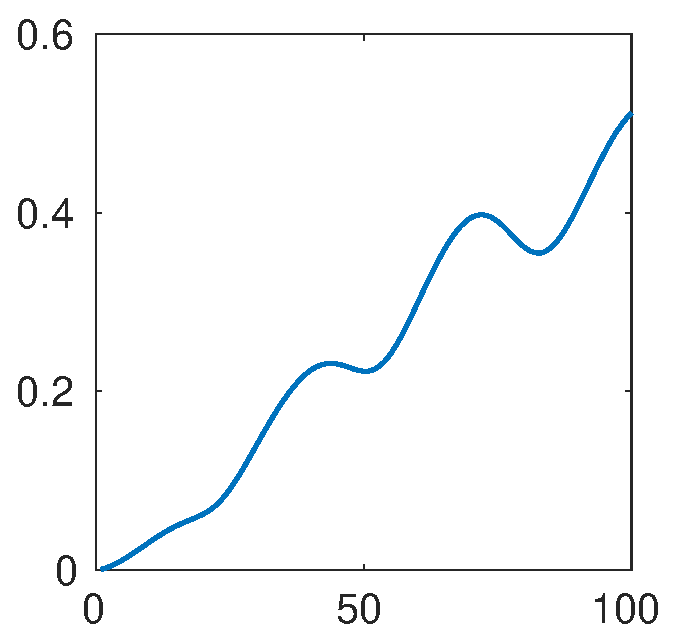
\includegraphics[height=0.22\textwidth]{figs/fig_guideBornk}
  }
\end{subcaptionbox}
\begin{subcaptionbox}{Born approximation of the inverse medium problem.
  \label{fig:bornInv}}[0.31\textwidth]{
  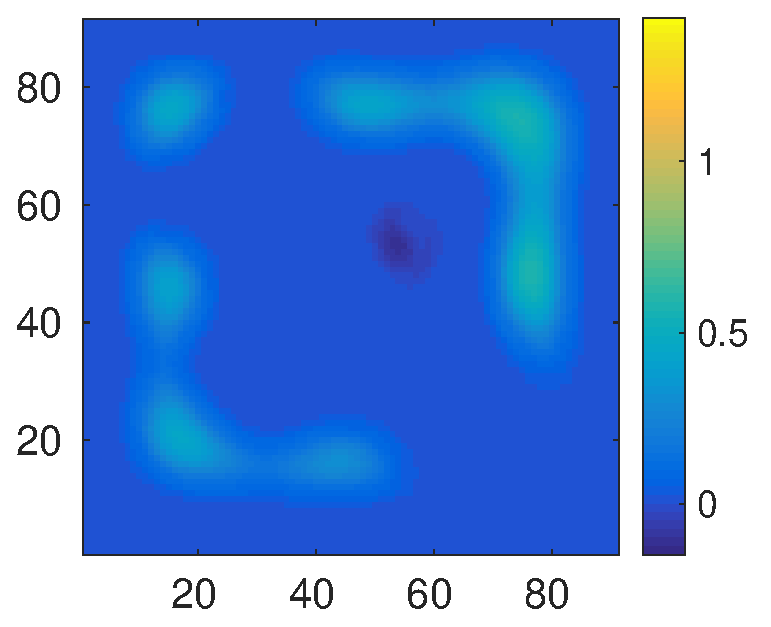
\includegraphics[height=0.22\textwidth]{figs/fig_guideBornInv_1000}
  }
\end{subcaptionbox}
\begin{subcaptionbox}{Error of the linearization.
  \label{fig:lin}}[0.31\textwidth]{
  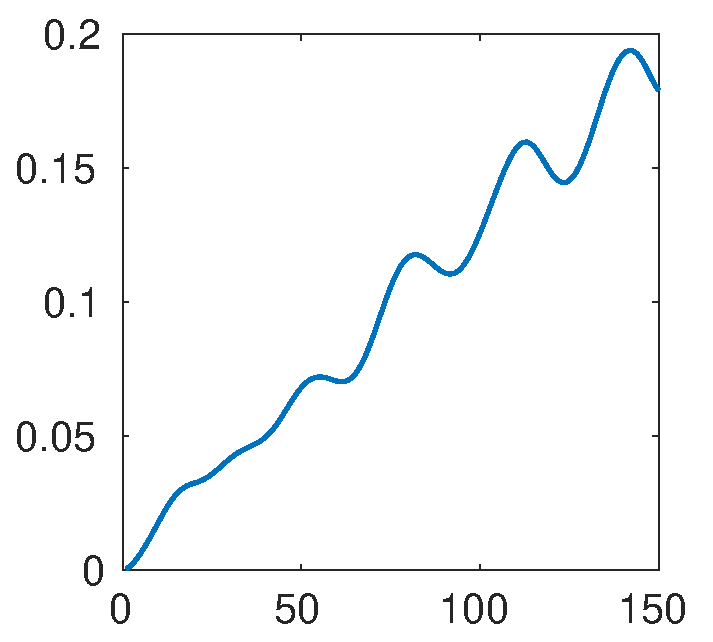
\includegraphics[height=0.22\textwidth]{figs/fig_guideLin}
  }
\end{subcaptionbox}
\caption{\subref{fig:born}~Relative error of the Born approximation (in comparison to the scattered field) in dependence of the wave number $k$ (in reciprocal meters). 
\subref{fig:bornInv}~Reconstruction of Fig.~\ref{fig:guide:recon1} with the Born approximation of the inverse medium problem using wave number $k = 70\,\si{m^{-1}}$ and $\textsf{seti.pdaN} = 1000$ inner iteration steps. Run time 1.4\,min, relative discrepancy $0.34$, relative error $0.78$. 
\subref{fig:lin}~Relative error of linearization $\F'(q)[h]+\F(q)$ in comparison to $\F(q+h)$ in dependence of the wave number $k$.}
\label{fig:bornAndLin}
\end{figure}

%%

\section*{Summary}
In this \emph{user guide} we have given installation instructions of the toolbox \IPscatt as well as a technical description. Further, we presented the key features of \IPscatt in a set of hands-on guides with step-by-step instructions. Finally, we demonstrated the suitability of \IPscatt for applications on some examples.

%%

\section*{Appendix}\label{sec:app}

For the reader's convenience this appendix contains introductions to the direct scattering problem and the implemented variational reconstruction scheme to repeat formulas from the \emph{algorithm paper} if we refer to them. For technical details we refer to~\cite{Buergel2017}. Furthermore, scattering simulation is one of the main components of \IPscatt. Therefore we summarize the essential formulas of the scattering simulation in Tab.~\ref{tab:forward} in continuous and discretized form as well as source code to build a connection between mathematical formulas and their implementation.

\paragraph{Introduction to the Direct Scattering Problem} For a wave number $k > 0$ the incident field $u^\Inc$ solves the Helm\-holtz equation
\begin{equation}\label{eq:HEQinc}
\Delta u^\Inc + k^2 u^\Inc = 0.
\end{equation}
The contrast is denoted by~$q$. Then the total field $u^\Tot$ solves the Helm\-holtz equation
\begin{equation}\label{eq:HEQ}
 \Delta u^\Tot + k^2 (1+q) u^\Tot = 0 \quad \text{ in } \R^d
\end{equation}
with $d = 2$ or $3$. 
The scattered field $u^\Sca$ is measured by means of the total field $u^\Tot$ via $u^\Sca = u^\Tot - u^\Inc$. The direct scattering problem (forward problem) is to find such a scattered field $u^\Sca$ to a given incident field and contrast.

For the consideration of the involved operators two domains are interesting: the computational domain~(CD), which is the square/cube around the circle/ball with radius $2R$, i.e. $\CD = [-2R,2R)^d$, and the region of interest~(ROI), which is the square/cube inside the small circle/ball with radius $R$, i.e. $\ROI = (-R/\sqrt{2},R/\sqrt{2})^d$.

The solution of the direct scattering problem is interesting in the latter domain, i.e. $u^\Sca$ in $\ROI$. Usually, this problem is solved by a reformulation: Find $u^\Sca$ solving the so-called Lippmann-Schwinger integral equation
\begin{equation}\label{eq:LSI}
 u^\Sca - V(q\cdot u^\Sca) = V(q\cdot u^\Inc) \quad \text{ for } x \in D,
\end{equation}
where the radiating volume potential is defined by
\begin{equation*}
 (Vf)(x) := k^2 \int_D \Phi(x-y)f(y)\ \d{y}, \quad x\in\R^d,
\end{equation*}
where $\Phi$ is the radiating fundamental solution of the Helmholtz equation,
\begin{equation}\label{eq:fundamental}
\Phi(x) = \frac{\im}{4} H_0^{(1)}(k|x|) \quad \text{ if } x \in \R^2\setminus\{0\},
\quad
\Phi(x) = \frac{1}{4\pi} \frac{\e^{\im k|x|}}{|x|} \quad \text{ if } x \in \R^3\setminus\{0\},
\end{equation}
where $H_0^{(1)}$ is the  Hankel function of the first kind and order zero, see~\cite[Ch.~9]{Abramowitz1965}. (Fast numerical solvers for the Lippmann-Schwinger integral equation are described for example in~\cite{Vainikko2000}.)

The direct scattering problem is solved by the forward operator~$\F$. To be more precise, the forward operator~$\F$ is the multi-static contrast-to-measurement operator, i.e. results in the scattered field at the receivers' positions for each of the incident fields. 

\paragraph{Introduction to the Variational Reconstruction Scheme} The inverse scattering problem is to find a contrast $q$ such that $\F(q)$ matches the data $\msdata^\delta$ with noise level $\delta$. The data can be synthetic data generated by adding noise to $\F(q)$ or real-world data.

The underlying variational reconstruction scheme of \IPscatt to solve this problem relies on the so-called primal-dual algorithm due to Pock, Bischof, Cremers and Chambolle, see~\cite{Pock2009, Chambolle2011}. To apply the primal-dual algorithm we linearize the forward operator $\F$.
Instead of the discrepancy $\|\F(q) - \msdata^\delta \|_\fro$ with the Frobenius norm $\|\cdot\|_\fro$ 
we consider 
$\|\F'(q)[h] + \F(q) - \msdata^\delta \|_\fro$ with the Fr\'echet derivative $\F'(q)$.
The functional to be minimized is in a simplified formulation
\begin{equation}\label{eq:minFuncSimple}
\min_{h \in \ROID} 
     \underbrace{
         \frac{1}{2}\|\F'(q)[h]+\F(q) - \msdata^\delta\|_\fro^2
         }_{=: f_\dis(h)}
   + \underbrace{\alpha \|q+h\|_1}_{=: f_\sparse(h)}
   + \underbrace{\beta \| \nabla (q+h) \|_1}_{=: f_\gra(h)}
   + \underbrace{
         \delta_{[a,b]}(\real(q+h) ) +
         \delta_{[c,d]}(\imag(q+h) )}_{=: f_\phy(h)}.
\end{equation}
The summands are the discrepancy of the linearized problem $f_\dis(h)$, the sparsity penalty $f_\sparse(h)$, the total variation penalty $f_\gra(h)$ and the physical bounds $f_\phy(h)$. 

Finally, the minimization scheme is to minimize~\eqref{eq:minFuncSimple} for a fixed contrast $q$ with the primal-dual algorithm, that we call \emph{inner iteration}. Afterwards, the \emph{outer iteration} is to update the contrast $q:= q+h$ before we minimize~\eqref{eq:minFuncSimple} again for the just redefined contrast $q$. Inner and outer iterations are repeated until the outer iteration is stopped by Morozov's discrepancy principle, i.e. if
\begin{equation}\label{eq:morozov}
\|\F(q) - \msdata^\delta \|_\fro / \|\msdata^\delta \|_\fro \leq \tau \delta \quad \text{with tolerance parameter } \tau > 1.
\end{equation}

\paragraph{Scattering Simulation} Scattering simulation is one of the main components of \IPscatt. Hence, we summarize the basic formulas of the direct scattering problem in Tab.~\ref{tab:forward} essentially in the chronological order of scattering. 
Without the claim of completeness we give them in continuous and discretized form as well as source code to build a connection between mathematical formulas and their implementation. 

% -- table: start --

\begin{longtable}{p{0.4cm} p{4.25cm} p{9.8cm} p{0.6cm}}
%
\hline\\*[-0.5em]
\multicolumn{3}{l}{\textsc{Single-layer potential for source points}}\\*
\formc & \highcol $\SL_{\TX \to \ROI} \colon L^2(\TX) \to L^2(\ROI)$, & \highcol $\displaystyle (\SL_{\TX \to \ROI}g)(x) := \int_{\TX} \Phi(x-y) g(y) \d{s(y)}, \quad x \in \ROI \setminus \TX$. & \ineqno{eq:SLC}\\*
\formd & $\SL_{N_\Inc,N_\ROI} \colon \TXD \to \ROID$, & $\displaystyle (\SL_{N_\Inc,N_\ROI} \underline{g}_{N_\Inc})(\ell) := \sum_{j = 1}^{N_\Inc} \omega_j^\Inc u_j^\Inc (x_\ell) \underline{g}_{N_\Inc}(j)$ \newline
with $u_j^\Inc(x) = \Phi(x-p_j)$, $j = 1, \ldots, N_\Inc$, in the case of source points at $p_j$ 
and approximations $\omega_j^\Inc = \textsf{seti.dSInc}$ of the infinitesimal element on $\TX$.\\*
\forms & $\textsf{SL} \colon \TXS \to \ROIS$, & \textsf{SL = dSInc(j)*incField(:,j)}\newline with $\textsf{dSInc}(j) = \omega_j^\Inc$ and $\textsf{incField} = u_j^\Inc(x) \underline{g}_{N_\Inc}$ in \textsf{mimo.m}.\\*
\formc & $\SL_{\S\to\ROI}$ & The single-layer potential in the case of plane waves.\\*
\\[-0.5em]
%
\hline\\*[-0.5em]
\multicolumn{3}{l}{\textsc{Volume potential operator}\footnote{More precisely, we consider the \emph{periodized} volume potential operator in this table.}}\\*
\formc & \highcol $V_{2R} \colon L^2(\CD) \to L^2(\CD)$, & \highcol $\displaystyle (V_{2R} f)(x) := \int_\CD \Phi_{2R}(x-y) f(y) \d{y}, \quad x \in \CD$. & \ineqno{eq:VPc}\\*
\formd & $V_\NROI \colon \ROID \to \ROID$, & $\displaystyle V_\NROI \underline{f}_\NROI:= \mathcal{R}_N \FFT_N^{-1} (\factorKernelNshi \pmul) \FFT_N \mathcal{E}_N \underline{f}_\NROI$.\\*
& & It is restricted to ROI and shifted because of the FFT.\\*
\forms & $\textsf{V} \colon \ROIS \to \ROIS$, & $\textsf{V = seti.k\^{}2.*helmholtz2Dr2r}$ with \textsf{helmholtz2Dr2r} computing\newline
\textsf{restrictCDtoROI(ifft2(reshape(seti.kHat,seti.nCD,seti.nCD).*...}\newline \textsf{fft2(extendROItoCD(fROI,seti.ROImask))),seti.ROImask)}. & \ineqno{eq:VPs}\\*
\\
\multicolumn{3}{l}{\textsc{Additional formulas for the volume potential operator}}\\*
 & $\mathcal{E} \colon L^2(\ROI) \to L^2(\CD)$, \newline $\mathcal{R} \colon L^2(\CD) \to L^2(\ROI)$ & 
\formc\,: $\mathcal{E}$ extends, $\mathcal{R}$ restricts and $\mathcal{E}^\ast = \mathcal{R}$.\newline
\formd\,: $\mathcal{E}_N \colon \ROID \to \CDD$ and $\mathcal{R}_N \colon \CDD\to\ROID$.\newline 
\forms\,: $\textsf{extendROItoCD} \colon \ROIS \to \CDS$, $\textsf{restrictCDtoROI} \colon \CDS \to \ROIS$.\\*
& $\FFT_N$, $\FFT_N^{-1}$ & \formd\ and \forms\,: $\FFT_N = \textsf{fft2}$, $\FFT_N^{-1} = \textsf{ifft2}$.\\*
& $\Phi_{2R}, \factorKernelNshi$, \textsf{seti.kHat} & \formd\ and \forms\,: The kernel $\Phi_{2R}(x)$ in the computational domain is $k^2 \Phi(x)$ if $x \in \overline{B_{2R}}$ and $0$ if $x \in \overline{\CD} \setminus \overline{B_{2R}}$. The shifted Fourier coefficients $\factorKernelNshi = S_N^{-1}([(4R)^{d/2} \, \hat{\Phi}_{2R}(j)]_{j \in \Z_N^d})$ of $\Phi_N$, where $S_N^{-1}$ represents the shifting, 
are defined as \textsf{seti.kHat} in \textsf{setKernel.m}. & \ineqno{eq:kHat}\\*
\\
\multicolumn{3}{l}{\textsc{Application of the volume potential operator $V_{2R}$ computing the scattered field $u^\Sca$}}\\*
\newline \forms & One incident field:\newline $\textsf{uScattROI}\colon \ROIS \to \ROIS$ & The routine \textsf{solveLippmannSchwinger(Vq, f, seti)} solves~\eqref{eq:LSI} 
computing \textsf{v} such that $\textsf{v} - \textsf{Vq(v)} = \textsf{f}$. Therefore a GMRES is used. 
For contrast \textsf{qROI} and incident field \textsf{uIncROI}, the scattered field is \textsf{uScattROI = solveLippmannSchwinger(@(x) V(qROI.*x), V(qROI.*uIncROI), seti)}.
& \ineqno{eq:appVol}\\*
\newline \forms & Multi-static:\newline \textsf{FFqROI} & \newline \textsf{FFqROI(:,j) = uScattROI} for each transmitter $j = 1, \ldots, N_\Inc$ in \textsf{mimo.m}. & \newline \ineqno{eq:FFqROI}\\*
\\
\multicolumn{3}{l}{\textsc{Adjoint of the volume potential operator}}\\*
\formc & $V_{2R}^\ast \colon L^2(\CD) \to L^2(\CD)$, & $\displaystyle (V_{2R}f)^\ast(x) := \int_\CD \overline{\Phi_{2R}(x-y)} f(y) \d{y}, \quad x \in \CD$.\\* 
\formd & $V_\NROI^\ast \colon \ROID \to \ROID$, & $\displaystyle V_\NROI^\ast \underline{f}_\NROI := \mathcal{R}_N \FFT_N^{-1} (\overline{\factorKernelNshi} \pmul ) \FFT_N \mathcal{E}_N \underline{f}_\NROI$.\\* 
\forms & $\textsf{VStar} \colon \ROIS \to \ROIS$, & \textsf{VStar = seti.k\^{}2.*helmholtz2Dr2rAdjoint}, cf.~\eqref{eq:VPs} using \textsf{seti.kHat'}.\\*
\\[-0.5em]
%
\hline\\*[-0.5em]
\multicolumn{3}{l}{\textsc{Solution-to-data operator (for near field data)}}\\*
\formc & \highcol $V_{\ROI \to \RX} \colon L^2(\ROI) \to L^2(\RX)$ & \highcol $\displaystyle (V_{\ROI \to \RX} f)(x):= k^2 \int_\ROI \Phi(x-y) f(y) \d{y}, \quad x\in\RX$. & \ineqno{eq:solToData}\\*
\formd & $V_{\NROI,N_\Sca} \colon \ROID \to \RXD$ & $\displaystyle (V_{\NROI,N_\Sca} \underline{f}_\NROI)(\ell)
  := \dV k^2 \sum\nolimits_{j\in\Z^d_N} \Phi(x_\ell-y^{(N)}_j) \underline{f}_{\NROI}(j)$\newline
  with points $y^{(N)}_j$ in ROI, the position $x_\ell$ of the $\ell$th receiver and the area/volume $\dV$ of the ROI's infinitesimal element (pixel/voxel). & \ineqno{eq:solToDataDis}\\*
\forms & $\textsf{uScattRX} \colon \ROIS \to \RXS$ & \textsf{uScattRX = seti.k\^{}2.*helmholtz2Dr2data(fROI, seti)} in \textsf{simo.m}, where \textsf{helmholtz2Dr2data} yields \textsf{(seti.measKer*fROI)*seti.dV} 
with $\textsf{seti.dV} = \dV$, $\textsf{fROI} = \underline{f}_\NROI$ and $\textsf{seti.measKer} = \Phi(x_\ell-y^{(N)}_j)$ for near field data defined in \textsf{setMeasKer.m}. 
 & \ineqno{eq:simo}\\*
\\
\multicolumn{3}{l}{\textsc{Adjoint of the solution-to-data operator (for near field data)}}\\*
\formc & $V_{\ROI \to \RX}^\ast \colon L^2(\RX) \to L^2(\ROI)$ & $\displaystyle (V_{\ROI\to\RX}^\ast f)(x):= k^2 \int_\RX \overline{\Phi(x-y)} f(y) \d{y}, \quad x\in\ROI$.\\*
\formd & $V_{\NROI,N_\Sca}^\ast \colon \RXD \to \ROID$, & $\displaystyle (V_{\NROI,N_\Sca}^\ast \underline{f}_{N_\Sca})(j) := \omega_j^\Sca\, k^2 \sum\nolimits_{\ell = 1, \ldots, N_\Sca} \overline{\Phi(x_\ell-y^{(N)}_j)} \underline{f}_{N_\Sca}(\ell)$.\newline
$\omega_j^\Sca = \textsf{seti.dSMeas}$: approximations of infinitesimal element of $\RX$. & \ineqno{eq:adjSolToDataDis}\\*
\forms & $\textsf{VGStar} \colon \RXS \to \ROIS$, & \textsf{VGStar = seti.k\^{}2.*helmholtz2Dr2dataAdjoint} under the use of \textsf{(seti.measKer')*(f.*seti.dSMeas)} in \textsf{helmholtz2Dr2dataAdjoint.m}.\\*
\\
\multicolumn{3}{l}{\textsc{Solution-to-data operator (for far field data)}}\\*
\formc \newline \forms & $V_{\ROI \to \S}$ & Operator as in~\eqref{eq:solToData},~\eqref{eq:simo}, but $\texttt{seti.measKer} = \gamma \exp(-\im k\langle y,\theta_\ell\rangle)$, where $y$ are points in ROI, $\theta_\ell$ is the direction of the $\ell$th receiver and $\gamma = \exp(\im \pi/4) / \sqrt{8 \pi k} \mathrm{\ if\ } x \in \R^2$ and $\gamma = 1/(4\pi) \mathrm{\ if\ } x \in \R^3$. & \ineqno{eq:solToDataFar}\\*
\\[-0.5em]
%
\hline\\*[-0.5em]
\multicolumn{3}{l}{\textsc{Lippmann-Schwinger solution operator}}\\*
\formc & \highcol $\LipS{q} \colon L^2(\ROI) \to L^2(\ROI)$ & \highcol $\LipS{q}:= (I-V_{2R}(q \, \cdot ))^{-1}$
& \ineqno{eq:LSIc}\\*
\formd & $\LipSd{\underline{q}} \colon \ROID \to \ROID$ & $\LipSd{\underline{q}} := (I - V_\NROI\pmulop{\underline{q}})^{-1}$\quad with $\underline{q} \in \ROID$.\\*
\\*
%
\formc & $\LipS{q}^\ast \colon L^2(\ROI) \to L^2(\ROI)$ & $\LipS{q}^\ast:= (I-(V_{2R}(q \, \cdot ))^\ast)^{-1}$\\*
\formd & $\LipSd{\underline{q}}^\ast \colon \ROID \to \ROID$ & $\LipSd{\underline{q}}^\ast := (I - (V_\NROI\pmulop{\underline{q}})^\ast)^{-1}$\quad with $\underline{q} \in \ROID$\\*
\forms & $\textsf{TStar} \colon \ROIS \to \ROIS$ & \textsf{TStar  = @(f) solveLippmannSchwinger(VqStar,f,seti)} under the use of \mbox{\textsf{VqStar = @(x) conj(qROI).*VStar(x)}}. Remember that \textsf{solveLippmannSchwinger} computes \textsf{v} such that $\textsf{v} - \textsf{VqStar(v)} = \textsf{f}$.\\*
\\[-0.5em]
%
\hline\\*[-0.5em]
\multicolumn{3}{l}{\textsc{Forward operator (multi-static contrast-to-measurement operator)}}\\*
\formc & \highcol $\F \colon L_{\imag \geq 0}^p (\ROI) \to \HS$ & \highcol $\displaystyle \F(q) := V_{\ROI \to \RX}(q \cdot) \LipS{q} \SL_{\TX\to\ROI}$. & \ineqno{eq:forward}\\*
& & Note that $\HS$ is the space of all Hilbert-Schmidt operators $\HS(L^2(\Gamma_\Inc),L^2(\Gamma_\Sca))$.\\*
\formd & $\underline{\F} \colon \ROID \to \C^{N_\Sca \times N_\Inc}$ & $\underline{\F}(\underline{q}) := V_{\NROI, N_\Sca}  \pmulop{\underline{q}} \LipSd{\underline{q}} \SL_{N_\Inc,\NROI}$.\\*
\newline \forms & One incident field:\newline 
$\textsf{uScattRX}\colon \ROIS \to \C^{N_\Sca}$ & \newline Compute \textsf{[uScattRX, uScattROI] = S(SL)} in \textsf{mimo.m}, where \textsf{S = @(s) simo(qROI, s, seti)} in \textsf{intOpsFuncs.m}. The task of \textsf{simo.m} is to compute $u^\Sca = \textsf{uScattROI}$ as in~\eqref{eq:appVol}, $\textsf{fROI = QU(uIncROI+uScattROI)} = q \pmul (u^\Inc + u^\Sca)$ and \textsf{uScattRX} as in~\eqref{eq:simo}. & \newline \ineqno{eq:forwardCodeSingle}\\*
\newline \forms & Multi-static:\newline
$\textsf{FFq}\colon \ROIS \to \C^{N_\Sca \times N_\Inc}$ & \newline \textsf{FFq(:,j) = uScattRX} for each transmitter $j = 1,\ldots, N_\Inc$ in \textsf{mimo.m}.
 & \newline \ineqno{eq:forwardCode}\\*
\\[-0.5em]
%
\hline\\*[-0.5em]
\multicolumn{3}{l}{\textsc{Fr\'{e}chet derivative of the forward operator}}\\*
\formc & \highcol $\F'(q) \colon L^2(\ROI) \to \HS$, & \highcol $\displaystyle \F'(q)[h]g = V_{\ROI \to \Gamma_\Sca} (I + (q \cdot) \LipS{q} V_{2R})(h \cdot) \LipS{q} \SL_{\Gamma_\Inc\to\ROI} g, \quad g\in L^2(\Gamma_\Inc)$.
 & \ineqno{eq:DFFqc}\\*
 & (cf.~\eqref{eq:forward} for $\HS$) & In finite-dimensional spaces the derivative $\F'(q)$ is represented by the Jacobian matrix denoted by $\underline{\F}'(\underline{q})$, see \cite[Sec.~3.6]{Buergel2017}:\\*
\formd & $\underline{\F}'(\underline{q})\colon \ROID \to \C^{N_\Sca \times N_\Inc}$ & $\displaystyle \underline{\F}'(\underline{q})[\underline{h}] = A_{\NROI,N_\Sca} \pmulop{\underline{h}} B_{\NROI,N_\Inc}$ for $\underline{h} \in \ROID$\newline 
$\begin{array}{llcl}
\text{with} & A_{\NROI,N_\Sca} & = & V_{\NROI,N_\Sca} \big(I + \pmulop{\underline{q}} \LipSd{\underline{q}} V_\NROI \big) \in \C^{N_\Sca \times \NROI},\\
& B_{\NROI,N_\Inc} &=& \LipSd{\underline{q}} \SL_{N_\Inc,\NROI} \in \C^{\NROI \times N_\Inc}.
\end{array}$
& \ineqno{eq:DFFqd}\\*
\forms & \textsf{DFFq} & \textsf{[JA,JB] = derivative(seti,qROI)} with $\textsf{JA} = A_{\NROI,N_\Sca}$ and $\textsf{JB} = B_{\NROI,N_\Inc}$ as well as $\textsf{qROI} = \underline{q}$, such that \textsf{DFFq = @(h) JA*diag(h)*JB} computes $\underline{\F}'(\underline{q})[h]$ by \textsf{DFFqh = DFFq(h)}.\\*
\\
%
\multicolumn{3}{l}{\textsc{Fr\'{e}chet derivative's adjoint of the forward operator}}\\*
\formd & $[\underline{\F}'(\underline{q})]^\ast\colon \C^{N_\Sca \times N_\Inc} \to \ROID$ & $\displaystyle [\underline{\F}'(\underline{q})]^\ast \underline{H} = \sum_{j = 1}^{N_\Sca} \sum_{\ell = 1}^{N_\Inc}  \underline{H}_{j,\ell}\, \overline{A_{\NROI,N_\Sca}(j,\cdot)} \, \overline{B_{\NROI,N_\Inc}(\cdot,\ell)}$ \quad for $\underline{H} \in \C^{N_\Sca \times N_\Inc}$. & \ineqno{eq:ADFFqc}\\*
& & Since discretizations of the domain space $L_{\imag \geq 0}^p$ and the inner product in $\HS$, see~\eqref{eq:forward}, take into account weights for physical reasons, there is an additional factor $\omega_j^\Sca/\dV$, see~\eqref{eq:solToDataDis} and~\eqref{eq:adjSolToDataDis}.\\*
\forms & \textsf{ADFFq} & \textsf{[ADFFq,seti] = adjOfDer(seti,qROI,FmeasDelta)} where $\textsf{ADFFq} = [\underline{\F}'(\underline{q})]^\ast [\underline{\F}(\underline{q}) - \msdata^\delta]$ with $\textsf{qROI} = \underline{q}$ and $\textsf{FmeasDelta} = \msdata^\delta$. 
Note that the adjoint applied to the defect results in the derivative of the least-squares error of the forward operator.\\*
\\[-0.5em]
%
\hline
\caption{The table contains the basic formulas of the direct scattering problem: the single-layer potential $\SL_{\TX \to \ROI}$, the volume potential operator $V$, the solution-to-data operator $V_{\ROI \to \RX}$ and the Lippmann-Schwinger solution operator $\LipS{q}$. In addition, for practical usage their adjoints are given as well as the forward operator~$\F$. Important ingredients of many reconstruction and optimization schemes are in the table too: the Fr\'{e}chet derivative $\F'(q)$ and its adjoint $[\F'(q)]^\ast$. \\
Without the claim of completeness they are presented in the order of continuous and discretized formulas and the source code highlighted by the symbols \formc, \formd\ and \forms. The notation $(f \cdot)$ is used to denote the operator of pointwise multiplication (with a function $f$). If we want to stress the pointwise multiplication we use the notation $f \cdot g$ in the continuous case and $f \pmul g$ in the discretized one. We underline a symbol to emphasize the discretization.}
\label{tab:forward}
\end{longtable}

% -- table: end --

%%

% \vspace*{-1em}

%%

% References
\begin{small}
\bibliography{input/references}
\bibliographystyle{alphaurl}
\end{small}

\end{document}
